%%%%%%%% ICML 2026 EXAMPLE LATEX SUBMISSION FILE %%%%%%%%%%%%%%%%%

\documentclass{article}

% Recommended, but optional, packages for figures and better typesetting:
\usepackage{microtype}
\usepackage{graphicx}
\usepackage{subcaption}
\usepackage{booktabs} % for professional tables

% hyperref makes hyperlinks in the resulting PDF.
% If your build breaks (sometimes temporarily if a hyperlink spans a page)
% please comment out the following usepackage line and replace
% \usepackage{icml2026} with \usepackage[nohyperref]{icml2026} above.
\usepackage{hyperref}


% Use the following line for the initial blind version submitted for review:
%\usepackage{icml2026}

% For preprint, use
\usepackage[preprint]{icml2026}

% If accepted, instead use the following line for the camera-ready submission:
% \usepackage[accepted]{icml2026}

\usepackage{amsmath}
\usepackage{amssymb}
\usepackage{mathtools}
\usepackage{amsthm}


% \usepackage{algorithm}
% %\usepackage{algorithmicx}
% \usepackage{algorithmic}

% \usepackage{algpseudocode}

% \usepackage{algorithm}
% \usepackage{algpseudocode}
% \usepackage{amsmath}


% if you use cleveref..
\usepackage[capitalize,noabbrev]{cleveref}


\usepackage{float}
\usepackage{cancel}





\usepackage{algorithm}
\usepackage{algorithmic}
\usepackage{amsmath}

\usepackage[algo2e]{algorithm2e}
\usepackage{hyperref}

%\usepackage[linesnumbered,algoruled,boxed,lined]{algorithm2e}

%%%%%%%%%%%%%%%%%%%%%%%%%%%%%%%%
% THEOREMS
%%%%%%%%%%%%%%%%%%%%%%%%%%%%%%%%
\theoremstyle{plain}
\newtheorem{theorem}{Theorem}[section]
\newtheorem{proposition}[theorem]{Proposition}
\newtheorem{lemma}[theorem]{Lemma}
\newtheorem{corollary}[theorem]{Corollary}
\theoremstyle{definition}
\newtheorem{definition}[theorem]{Definition}
\newtheorem{assumption}[theorem]{Assumption}
\theoremstyle{remark}
\newtheorem{remark}[theorem]{Remark}

% Todonotes is useful during development; simply uncomment the next line
%    and comment out the line below the next line to turn off comments
%\usepackage[disable,textsize=tiny]{todonotes}
\usepackage[textsize=tiny]{todonotes}


\usepackage{amsmath,amssymb,amsfonts,bm}
\usepackage{mathtools}


\usepackage{graphicx}
\usepackage{subcaption}

\usepackage{tikz} 

\usetikzlibrary{arrows.meta,positioning,calc}



\newcommand{\va}{\boldsymbol{a}}
\newcommand{\mA}{\boldsymbol{A}}
\newcommand{\vb}{\boldsymbol{b}}
\newcommand{\mB}{\boldsymbol{B}}
\newcommand{\vc}{\boldsymbol{c}}
\newcommand{\mC}{\boldsymbol{C}}
\newcommand{\vd}{\boldsymbol{d}}
\newcommand{\mD}{\boldsymbol{D}}

\newcommand{\mE}{\boldsymbol{E}}
\newcommand{\ve}{\boldsymbol{e}}
\newcommand{\mF}{\boldsymbol{F}}
\newcommand{\vf}{\boldsymbol{f}}
\newcommand{\mG}{\boldsymbol{G}}
\newcommand{\vg}{\boldsymbol{g}}
\newcommand{\mH}{\boldsymbol{H}}
\newcommand{\vh}{\boldsymbol{h}}
\newcommand{\mI}{\boldsymbol{I}}
\newcommand{\vi}{\boldsymbol{i}}
\newcommand{\mJ}{\boldsymbol{J}}
\newcommand{\vj}{\boldsymbol{j}}
\newcommand{\mK}{\boldsymbol{K}}
\newcommand{\vk}{\boldsymbol{k}}
\newcommand{\mL}{\boldsymbol{L}}
\newcommand{\vl}{\boldsymbol{l}}
\newcommand{\mM}{\boldsymbol{M}}
\newcommand{\vm}{\boldsymbol{m}}
\newcommand{\mN}{\boldsymbol{N}}
\newcommand{\vn}{\boldsymbol{n}}
\newcommand{\mO}{\boldsymbol{O}}
\newcommand{\vo}{\boldsymbol{o}}
\newcommand{\mP}{\boldsymbol{P}}
\newcommand{\vp}{\boldsymbol{p}}
\newcommand{\mQ}{\boldsymbol{Q}}
\newcommand{\vq}{\boldsymbol{q}}
\newcommand{\mR}{\boldsymbol{R}}
\newcommand{\vr}{\boldsymbol{r}}
\newcommand{\mS}{\boldsymbol{S}}
\newcommand{\vs}{\boldsymbol{s}}
\newcommand{\mT}{\boldsymbol{T}}
\newcommand{\vt}{\boldsymbol{t}}
\newcommand{\mU}{\boldsymbol{U}}
\newcommand{\vu}{\boldsymbol{u}}
\newcommand{\mV}{\boldsymbol{V}}
\newcommand{\vv}{\boldsymbol{v}}
\newcommand{\mW}{\boldsymbol{W}}
\newcommand{\vw}{\boldsymbol{w}}
\newcommand{\mX}{\boldsymbol{X}}
\newcommand{\vx}{\boldsymbol{x}}
\newcommand{\mY}{\boldsymbol{Y}}
\newcommand{\vy}{\boldsymbol{y}}
\newcommand{\mZ}{\boldsymbol{Z}}
\newcommand{\vz}{\boldsymbol{z}}


\newcommand{\mDiag}{\mathrm{Diag}}
\newcommand{\norm}[1]{\left\lVert #1 \right\rVert_2}

\newcommand{\vgamma}{\boldsymbol{\gamma}}


\newcommand{\mPsi}{\boldsymbol{\Psi}}

\newcommand{\valpha}{\boldsymbol{\alpha}}

\newcommand{\cty}[1]{\textcolor{magenta}{{[cty: #1]}}\xspace}
\newcommand{\qxb}[1]{\textcolor{red}{{[qxb: #1]}}\xspace}





% Capitalize autoref
\renewcommand{\sectionautorefname}{Section}
\renewcommand{\subsectionautorefname}{Subsection}
\renewcommand{\subsubsectionautorefname}{Subsubsection}
\renewcommand{\appendixautorefname}{Appendix}
\renewcommand{\algorithmautorefname}{Algorithm}

% Attempt to make hyperref and algorithmic work together better:
%\newcommand{\theHalgorithm}{\arabic{algorithm}}




% The \icmltitle you define below is probably too long as a header.
% Therefore, a short form for the running title is supplied here:
\icmltitlerunning{SimpleGPT: Improving GPT via A Simple Normalization Strategy}


\begin{document}



\twocolumn[
  \icmltitle{SimpleGPT: Improving GPT via A Simple Normalization Strategy}

  % It is OKAY to include author information, even for blind submissions: the
  % style file will automatically remove it for you unless you've provided
  % the [accepted] option to the icml2026 package.

  % List of affiliations: The first argument should be a (short) identifier you
  % will use later to specify author affiliations Academic affiliations
  % should list Department, University, City, Region, Country Industry
  % affiliations should list Company, City, Region, Country

  % You can specify symbols, otherwise they are numbered in order. Ideally, you
  % should not use this facility. Affiliations will be numbered in order of
  % appearance and this is the preferred way.
  \icmlsetsymbol{equal}{*}
  \icmlsetsymbol{comp}{$\dagger$}

  \begin{icmlauthorlist}
    \icmlauthor{Marco Chen}{yyy,equal}
    \icmlauthor{Xianbiao Qi}{xxx,equal,comp}
    \icmlauthor{Yelin He}{xxx}
    \icmlauthor{Jiaquan Ye}{xxx}
    \icmlauthor{Rong Xiao}{xxx}

  \end{icmlauthorlist}

  %\icmlaffiliation{yyy}{Tsinghua University, Beijing, China}
  %\icmlaffiliation{xxx}{Intellifusion Inc., Shenzhen, China}
  \icmlaffiliation{yyy}{Tsinghua University}
  \icmlaffiliation{xxx}{Intellifusion Inc.}

  \icmlcorrespondingauthor{Xianbiao Qi}{qixianbiao@gmail.com}


  % You may provide any keywords that you find helpful for describing your
  % paper; these are used to populate the "keywords" metadata in the PDF but
  % will not be shown in the document
  \icmlkeywords{Machine Learning, ICML}

  \vskip 0.3in
]




% this must go after the closing bracket ] following \twocolumn[ ...

% This command actually creates the footnote in the first column listing the
% affiliations and the copyright notice. The command takes one argument, which
% is text to display at the start of the footnote. The \icmlEqualContribution
% command is standard text for equal contribution. Remove it (just {}) if you
% do not need this facility.

% Use ONE of the following lines. DO NOT remove the command.
% If you have no special notice, KEEP empty braces:
%\printAffiliationsAndNotice{}  % no special notice (required even if empty)
% Or, if applicable, use the standard equal contribution text:
\printAffiliationsAndNotice{\icmlEqualContribution}

\begin{abstract}
    In this work, we revisit Transformer optimization through the lens of second-order geometry and establish a direct connection between architectural design, activation scale, the Hessian matrix, and the maximum tolerable learning rate. We introduce a simple normalization strategy, termed SimpleNorm, which stabilizes intermediate activation scales by construction. Then, by analyzing the Hessian of the loss with respect to network activations, we theoretically show that SimpleNorm significantly reduces the spectral norm of the Hessian, thereby permitting larger stable learning rates. We validate our theoretical findings through extensive experiments on large GPT models at parameter scales 1B, 1.4B, 7B and 8B. Empirically, SimpleGPT, our SimpleNorm-based network, tolerates learning rates 3$\times$-10$\times$ larger than standard convention, consistently demonstrates strong optimization stability, and achieves substantially better performance than well-established baselines. Specifically, when training 7B-scale models for 60K steps, SimpleGPT achieves a training loss that is 0.08 lower than that of LLaMA2 with QKNorm, reducing the loss from 2.290 to 2.208. Our source code will be released at \url{https://github.com/Ocram7/SimpleGPT}.
\end{abstract}


\section{Introduction}
% Efforts to enhance the reasoning capabilities of Large Language Models (LLMs) primarily rely on training paradigms such as Supervised Fine-Tuning (SFT)~\citep{achiam2023gpt}, Direct Preference Optimization (DPO)~\citep{rafailov2023direct}, and Reinforcement Learning (RL)~\citep{schulman2017proximal, guo2025deepseek, zeng2025simplerl}, which enable LLMs to iteratively interact with data, essentially engaging in trial-and-error learning to acquire problem-solving skills. This learning paradigm can be conceptualized as self-learning for LLMs. However, real-world knowledge acquisition is rarely isolated~\citep{bloembergen2015evolutionary, canese2021multi}. Humans continuously engage in knowledge exchange through collaborative learning, such as peer discussions in classroom settings. For human learning, while \textit{single-agent learning} (self-learning) forms the foundation, \textit{multi-agent learning} represents a more advanced and effective paradigm~\citep{zambrano2019effects}. Therefore, a critical question naturally arises: Can multi-agent learning enable LLMs to acquire deeper knowledge and exhibit superior reasoning compared to single-agent approaches?

Efforts to enhance the reasoning capabilities of Large Language Models (LLMs) have largely relied on training paradigms such as Supervised Fine-Tuning (SFT)~\citep{achiam2023gpt}, Preference Learning (PL)~\citep{rafailov2023direct}, and Reinforcement Learning (RL)~\citep{schulman2017proximal, guo2025deepseek, zeng2025simplerl}. 
These methods allow LLMs to iteratively interact with data and refine their behavior, essentially engaging in trial-and-error learning to acquire problem-solving skills, which can be viewed as self-learning for LLMs. 
However, real-world knowledge acquisition is rarely an isolated activity~\citep{bloembergen2015evolutionary, canese2021multi}. Humans continuously exchange knowledge through collaborative learning, as in peer discussions within classroom settings. While \textit{single-agent learning} (self-learning) serves as the foundation of human education, \textit{multi-agent learning} represents a more advanced and often more effective paradigm: multiple learners bring diverse perspectives, challenge each other's reasoning, and provide mutual feedback, ultimately leading to deeper understanding and more robust solutions~\citep {kahveci2007interactive, hsiung2012effectiveness, zambrano2019effects, mende2021individual}. The same principle suggests that multi-agent learning can benefit LLMs\footnote{In our paper, ``Agent'' and ``LLM'' refer to the same entity/concept}: by exposing models to diverse reasoning strategies and peer-based feedback, it may help them overcome individual blind spots and develop stronger problem-solving abilities. 
% This naturally raises a central question: \textit{Can multi-agent learning enable LLMs to acquire deeper knowledge and demonstrate superior reasoning in single-agent settings?}

Recent studies have explored multi-agent learning. For example, MALT~\citep{motwani2024malt} designs a sequential multi-agent system (MAS) consisting of Generator, Verifier, and Refiner agents, each independently trained to sample specialized trajectories. ReMA~\citep{wan2025rema} introduces a hierarchical framework with a high-level agent responsible for problem decomposition and a low-level agent for concrete step implementation, trained alternately to achieve complementary expertise. MAPoRL~\citep{park2025maporl} proposes a Post-Co-Training framework to enhance collaboration alignment through debate. However, during inference, these methods are required to re-execute the MAS to obtain final solutions, a process misaligned with human cognition, where individuals improve reasoning through peer interactions and subsequently solve problems independently.

% While effective at improving inter-agent collaboration, these approaches mainly emphasize strengthening the MAS as a whole, rather than directly improving the independent reasoning abilities of individual LLMs.


\begin{figure}[t]
\begin{center}
%\framebox[4.0in]{$\;$}
\includegraphics[width=1.0\linewidth]{iclr2026/figures/background.pdf}
\end{center}
% \vspace{-14pt}
\caption{Conceptual comparison of ILR, existing Multi-agent Learning, and Single-agent Learning. ILR enhances LLMs' independent reasoning ability through Dynamic Interaction and Perception Calibration at training time, and LLMs can resolve questions independently at inference time. 
}
% \vspace{-10pt}
\label{fig: background}
\end{figure}

In this paper, we address this gap by treating each agent as an autonomous entity and investigating whether multi-agent learning can enhance an LLM's individual problem-solving capacity (see Figure~\ref{fig: background}). We propose \textbf{ILR} (\textbf{I}nteractive \textbf{L}earning for LLM \textbf{R}easoning), a co-learning framework consisting of two key components: \textit{Dynamic Interaction} and \textit{Perception Calibration}. 

% Dynamic Interaction simulates human discussion patterns. For ``Dynamic'', when confronted with complex problems, different human individuals tend to cooperate, whereas for simpler problems, they would like to compete to find out whose solution is more efficient and advantageous. To simulate this behavior, an LLM first conducts difficulty measurement of the question by self-ranking, then calculates its probability of independently solving the problem based on  Item Response Theory (IRT)~\citep{benedetto2023survey, cai2016item}. When the probability of independent resolution is low, the LLM opts for cooperation; otherwise, it chooses competition. For ``Interaction'', we design a novel \textbf{Idea3} framework that comprises three sequential stages: Idea Sharing, Idea Analysis, and Idea Fusion, which corresponds to sharing LLM's ideas, analyzing another LLM's ideas, and synthesizing all content to generate novel ideas. 

The \textit{Dynamic Interaction} module simulates human discussion. For ``Dynamic'', when confronted with complex problems, humans tend to cooperate, whereas for simpler problems, they often compete to identify the most efficient solution~\citep{richard2002cooperation,schneider2011cooperation}. To emulate this behavior, an LLM estimates question difficulty through self-ranking and applies Item Response Theory~\citep{cai2016item, benedetto2023survey} to calculate the probability of solving it independently. If the probability is low, the model engages in cooperation; otherwise, it chooses competition. For ``Interaction'', we design a novel \textbf{Idea3} framework, comprising three sequential stages: Idea Sharing (each LLM proposes its own solution), Idea Analysis (each LLM analyzes and reflects on the peer's solution), and Idea Fusion (the insights are synthesized into a refined and potentially novel solution). Following Dynamic Interaction, the \textit{Perception Calibration} module is applied. Prior work~\citep{ma2024coevolving, park2025maporl} has shown that incorporating tailored reward signals can effectively guide LLMs toward better multi-agent learning. Instead of relying on predefined hyperparameters for reward shaping, we introduce a fully automated mechanism that integrates one LLM's reward distribution characteristics, derived from answer group sampling on the same input, into another LLM's reward function. We then employ Group Relative Policy Optimization (GRPO)~\citep{shao2024deepseekmath} to update each LLM based on calibrated rewards. This plug-and-play calibration allows LLMs to perceive the quality of peer-generated solutions and adapt their reasoning accordingly.


% Following Dynamic Interaction, we employ the Group Relative Policy Optimization (GRPO) algorithm~\citep{shao2024deepseekmath} to train each LLM. Previous works~\citep{park2025maporl, ma2024coevolving} indicate that incorporating specific signals in the reward can effectively steer LLMs towards better multi-agent learning. In contrast to their approach of using predefined hyperparameters for reward shaping, our Perception Calibration module utilizes a fully automated arithmetic operation to integrate one LLM's reward distribution characteristics, which can be obtained based on the answer group sampling from the same input question, into another LLM's reward function. Subsequently, each LLM undergoes GRPO training based on these calibrated rewards. Perception Calibration operates as a simple yet effective, plug-and-play component that enables LLMs to perceive the quality of solutions generated by other LLMs in multi-agent learning systems.


% We conduct experiments across two model series with different scales to validate the effectiveness of ILR, including Llama-3.1-8B-Instruct~\citep{dubey2024llama}, Qwen2.5-7B-Instruct~\citep{team2024qwen2}, and Qwen2.5-14B-Instruct~\citep{team2024qwen2}. Given the substantial computational costs associated with multi-agent training, we organize these three models into three pairwise groups. To maintain simplicity in the training, we only adopt MATH~\citep{hendrycks2021measuring} as the training dataset and evaluate performance across six distinct benchmarks. 

We evaluate the effectiveness of ILR on two model families of different scales: Llama-3.1-8B-Instruct~\citep{dubey2024llama}, Qwen2.5-7B-Instruct, and Qwen2.5-14B-Instruct~\citep{team2024qwen2}. For multi-agent training, we pair these three models to form three different groups. Following~\citep{zeng2025simplerl}, we use MATH~\citep{hendrycks2021measuring} as the training dataset and assess performance across five mathematical reasoning benchmarks and a code benchmark. Experimental results demonstrate that ILR consistently outperforms traditional single-agent learning, achieving improvements of up to 5\% over the strongest baseline models. Our investigation further reveals two findings: (1) Idea3 enhances the robustness of stronger LLMs during multi-agent inference scenarios. Analyzing and reflecting on the peer's solutions reduces the probability of being misled by weaker LLMs when exchanging information.
(2) Dynamically determining interaction types can boost the efficacy of multi-agent learning and surpass pure cooperation or competition strategies.
% \qcw{add more detailed explanations and insights when discussing the results. The experimental results demonstrate the superiority of ILR compared to single-agent learning, achieving an average improvement of 2\% points over the strongest baseline across all three models. We further investigate the advantages conferred by the Idea3 interaction framework in multi-agent inference scenarios.} 
Our main contributions are summarized as follows:

% \begin{itemize}
\begin{itemize}[leftmargin=*,labelsep=2mm]
    \item Unlike prior multi-agent learning approaches that primarily focus on improving inter-agent collaboration to strengthen overall system performance, to the best of our knowledge, we are the first to investigate whether multi-agent learning can more effectively enhance an LLM's independent reasoning capability compared to single-agent learning.
    \item Inspired by human interaction, we design a novel multi-agent learning framework ILR with Dynamic Interaction and Perception Calibration. The former adaptively selects cooperation or competition strategies and engages LLMs in Idea3 to gain better solutions. The latter enables LLMs to perceive the peer's performance and enhance the cohesion of multi-agent interactions.
    \item Through extensive experiments and analysis, we demonstrate the effectiveness of ILR over self-learning baselines. We further discover that Idea3 enhances the robustness of advanced LLMs by enabling them to analyze and reflect on the peer's solutions, and dynamic interaction strategies improve multi-agent learning by adapting to question difficulty.
\end{itemize}


\section{Related Work}\label{sec:related_works}
\paragraph{Normalization methods.}
Normalization has long been a central tool for stabilizing optimization and improving convergence in deep networks. Batch Normalization (BN)~\cite{batch_normalization_ioffe2015batch} normalizes activations using mini-batch statistics and has been widely successful in convolutional architectures, but its behavior can depend on batch size and distributed synchronization. Layer Normalization (LN)~\cite{layernorm_ba2016layer} and its variants remove batch dependence by computing statistics across features within each sample and have become the standard in Transformers. Related methods such as Instance Normalization (IN)~\cite{instance_norm_ulyanov2016instance}, Group Normalization (GN)~\cite{group_norm_wu2018group}, RMSNorm~\cite{rmsnorm_zhang2019root}, and nGPT~\cite{ngpt_loshchilov2024ngpt} further tailor normalization to specific architectural or efficiency constraints.


\textbf{Normalization Placement in Transformers.}
Beyond the choice of normalization operator, its \emph{placement} within Transformer blocks plays a critical role in optimization stability. The original Transformer architecture adopted post-normalization (PostNorm), in which normalization follows residual addition~\cite{transformer_vaswani2017attention}. Subsequent large-scale practice shifted toward pre-normalization (PreNorm), placing normalization before attention and MLP sublayers to improve trainability in deep networks~\cite{prenorm_wang2019learning}.

Recent work further systematizes normalization placement and explores additional insertion points. Deeply Normalized Transformer (DNT)~\cite{dnt_qi2025dnt} categorizes multiple strategies—including InputNorm, PreNorm, MidNorm, PostNorm, and QKNorm—and motivates them through a Jacobian- and gradient-stability analysis. DNT ultimately combines InputNorm, PreNorm, MidNorm, and QKNorm, while avoiding PostNorm due to its potential training instabilities. Among these placements, QK normalization (QKNorm)~\cite{qk_norm_henry2020query} specifically targets the attention mechanism, stabilizing the geometry of query–key interactions and mitigating softmax saturation.

By treating normalization as a design space over both operator and location, these works emphasize that stability and conditioning can be targeted at specific architectural subcomponents, rather than only at block outputs. As model depth increases, normalization also interacts with residual pathways and initialization. DeepNorm~\cite{deepnorm_wang2022deepnet}, for example, modifies residual scaling and initialization to bound parameter updates and control dynamical growth with depth, complementing normalization-placement strategies.


\textbf{Normalization-free Transformers.}
Motivated by the cost/complexity of normalization and the desire for simpler training dynamics, recent work questions whether explicit normalization is necessary in Transformers.
\emph{Transformers without Normalization} shows that replacing normalization layers with a simple point-wise nonlinearity, {Dynamic Tanh (DyT)}~\cite{dyt_zhu2025transformers}, can match normalized baselines across tasks, suggesting that an appropriate bounded nonlinearity can provide much of the stability typically attributed to LN/RMSNorm. 
Building on this, \emph{Stronger Normalization-Free Transformers}~\cite{stronger_norm_chen2025stronger} studies the design of point-wise functions more broadly and reports improved normalization-free performance via a searched function family (e.g., \(\mathrm{Derf}\)), outperforming LN/RMSNorm/DyT across multiple domains. Despite being framed as normalization-free, these approaches fundamentally operate by controlling the norm of activations through bounded transformations, and can therefore be viewed as a form of implicit normalization.



\textbf{Positioning of our work.}
While our method can be viewed as a study of normalization placement in Transformers, its key distinction lies in explicitly linking architectural design to second-order optimization geometry. Rather than motivating normalization heuristically or empirically, we analyze how local normalization immediately following linear mappings stabilizes activation scale and, in turn, constrains the spectral norm of the Hessian and leads to a smoother optimization landscape. This perspective yields a principled characterization of the maximum tolerable learning rate and provides a unified theoretical explanation for optimization stability in large Transformer models.
\section{Preliminaries}
We consider the unconstrained convex optimization problem
$\min_{\vx \in \mathbb{R}^d} f(\vx),$
where \(f:\mathbb{R}^d \to \mathbb{R}\) is \emph{differentiable}.  

\subsection{Convex and Smoothed Optimization}

\textbf{Lipschitz gradient smoothness.}
If \(f\) is twice differentiable, its second-order Taylor expansion at point $\vx$ is
\begin{align*}
    f(\vy)
\approx f(\vx)
&+ \langle \nabla f(\vx), \vy - \vx \rangle \\
&+ \frac{1}{2} (\vy - \vx)^\top \nabla^2 f(\vx) (\vy - \vx).
\end{align*}
The second-order term captures the local curvature.

\begin{definition}[$\beta$-smoothness]
The function \(f\) is said to be \(\beta\)-smooth if
\[
\|\nabla f(\vy)-\nabla f(\vx)\|_2 \le \beta \|\vy-\vx\|_2,
\forall \vy,\vx.
\]
\end{definition}

For convex and differentiable functions, \(\beta\)-smoothness is equivalent to the following quadratic upper bound:
\[
f(\vy) \le f(\vx) + \langle \nabla f(\vx), \vy-\vx \rangle
+ \frac{\beta}{2}\|\vy-\vx\|_2^2,
 \forall \vy,\vx .
\]
This inequality plays a central role in step-size (learning rate) selection for optimization methods.

\textbf{Gradient descent and learning rate.}
Consider the standard gradient descent iteration
\[
\vx_{k+1} = \vx_k - \eta \nabla f(\vx_k),
\]
where \(\eta>0\) is the learning rate. We wish to understand how the choice of \(\eta\) depends on the smoothness constant \(\beta\), and how this choice affects convergence.

\textbf{Descent condition.}
Evaluating the quadratic upper bound with
$\vy = \vx_{k+1} = \vx_k - \eta \nabla f(\vx_k)$ and $\vx = \vx_{k}$, we obtain
\[
f(\vx_{k+1})
\le f(\vx_k)
- \eta \|\nabla f(\vx_k)\|_2^2
+ \frac{\beta \eta^2}{2}\|\nabla f(\vx_k)\|_2^2 .
\]
Rearranging terms gives
\[
f(\vx_{k+1})
\le f(\vx_k)
- \left(\eta - \frac{\beta \eta^2}{2}\right)
\|\nabla f(\vx_k)\|_2^2 .
\]

A sufficient condition for monotone decrease of the objective is therefore
\begin{equation}
    0 < \eta \le \frac{2}{\beta}.
\end{equation}
This bound characterizes the \emph{stability region} of gradient descent for convex \(\beta\)-smooth functions. $\frac{2}{\beta}$ is usually known as the maximum tolerable learning
rate. 


For convex $\beta$-smooth problems, among all fixed learning rates that ensure descent, the canonical choice is typically $\eta = \frac{1}{\beta}$. This choice balances progress and stability and leads to the sharpest worst-case guarantees.

\subsection{Gradient and Hessian of a Linear Projection}
Given linear projection $\vy=\mW\vx$ and loss function $\ell$, the gradient and Hessian of $\ell$ with respect to $\vy$ are,
\[
\vg_{\vy} := {\frac{\partial \ell}{\partial \vy}}^{\top},
\qquad
\mH_{\vy\vy} := \frac{\partial^2 \ell}{\partial \vy \partial \vy^\top}.
\]
The Jacobian of $\vy$ with respect to $\vx$ is
$\mJ_{\vx}^{\vy}  = \frac{\partial \vy}{\partial \vx} = \mW.$
Hence, according to the chain rule, we have
\[
\vg_{\vx} = {\frac{\partial \ell}{\partial \vx}}^{\top}
=
{\mJ_{\vx}^{\vy}}^\top \vg_{\vy}
=
\mW^\top \vg_{\vy},
\]
and the Hessian matrix with respect to $\vx$ is
\begin{equation}
    \mH_{\vx\vx} = \frac{\partial^2 \ell}{\partial \vx \partial \vx^\top}
=
{\mJ_{\vx}^{\vy}}^\top \mH_{\vy\vy} \mJ_{\vx}^{\vy}
=
\mW^\top \mH_{\vy\vy} \mW.
\end{equation}

\section{Methodology}

\begin{figure*}[ht]
\tiny
     \centering
     	\begin{subfigure}[b]{\textwidth}
        \centering

            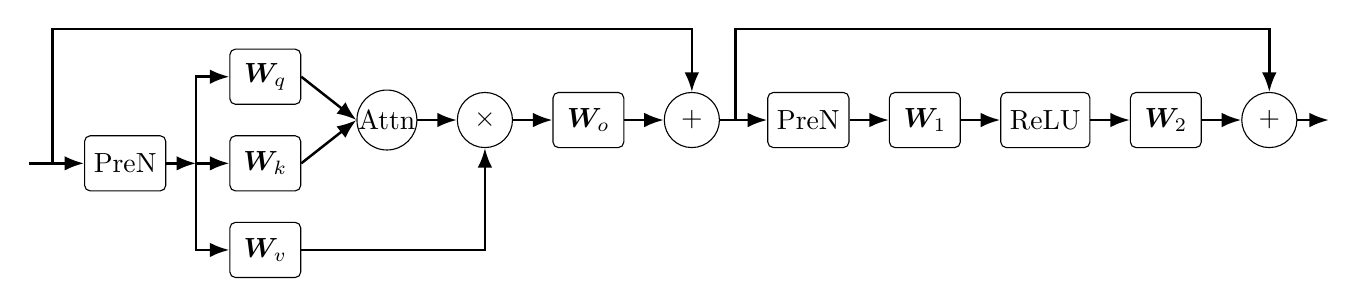
\begin{tikzpicture}[
                font=\normalsize,
                >=Latex,
                node distance=10mm and 14mm,
                block/.style={draw, rounded corners=2pt, minimum height=7mm, minimum width=9mm, align=center},
                smallblock/.style={draw, rounded corners=2pt, minimum height=7mm, minimum width=9mm, align=center},
                circ/.style={draw, circle, minimum size=7mm, inner sep=0pt},
                plus/.style={circ},
                mult/.style={circ},
                line/.style={-Latex, line width=0.9pt},
            ]
            
            % ----- Left part (Attention) -----
            
            \node[block] (pren1) {PreN};
            
            
            \node[smallblock, right=8mm of pren1, yshift=11mm] (wq) {$\mW_q$};
            
            \node[smallblock, right=8mm of pren1]     (wk) {$\mW_k$};
            \node[smallblock, right=8mm of pren1, yshift=-11mm]    (wv) {$\mW_v$};
            
            \node[circ, right=7mm of wk, yshift=5.5mm] (att) {Attn};
            
            \node[mult, right=5mm of att] (mul) {$\times$};
            
            \node[smallblock, right=5mm of mul] (wo) {$\mW_o$};
            
            \node[plus, right=5mm of wo] (add1) {$+$};
            
            % wiring: pren1 splits to wq,wk,wv
            \draw[line] (pren1) -- (9mm,0) coordinate (split1);
            \draw[line] (split1) |- (wq.west);
            \draw[line] (split1) |- (wk.west);
            \draw[line] (split1) |- (wv.west);
            
            % wq,wk -> att
            \draw[line] (wq.east) -- (att.west);
            \draw[line] (wk.east) -- (att.west);
            
            % att -> mul (top input)
            \draw[line] (att.east) -- (mul.west);
            
            % wv -> mul (bottom input)
            \draw[line] (wv.east) -| ($(mul.south)+(0,-6mm)$) -- (mul.south);
            % mul -> wo -> add1
            \draw[line] (mul.east) -- (wo.west);
            \draw[line] (wo.east) -- (add1.west);
            
            % local residual into add1 (from pren1 input stream)
            %\draw[line] (pren1.west) ++(-7mm,0) coordinate (x0);
            %\draw[line] (x0) -- (pren1.west);

            %\draw[line] (pren1.west) ++(-7mm,0) coordinate (x0);
            \draw[line] (pren1.west) ++(-7mm,0) coordinate (x0) -- (pren1.west);
            \draw[line] (x0)+(3mm,0) |- ($(add1.north)+(0,8mm)$) -- (add1.north);



            
            
            % ----- Right part (MLP) -----
            \node[block, right=6mm of add1] (pren2) {PreN};
            \node[smallblock, right=5mm of pren2] (w1) {$\mW_1$};
            \node[block, right=5mm of w1] (relu) {ReLU};
            \node[smallblock, right=5mm of relu] (w2) {$\mW_2$};
            \node[plus, right=5mm of w2] (add2) {$+$};
            
            % main forward
            \draw[line] (add1.east)  -- (pren2.west);
            \draw[line] (pren2.east) -- (w1.west);
            \draw[line] (w1.east) -- (relu.west);
            \draw[line] (relu.east) -- (w2.west);
            \draw[line] (w2.east) -- (add2.west);
            \draw[line] (add2.east) -- ++(4mm,0);
            
            % residual into add2 (from add1 output)
            \draw[line] (add1.east)+(2mm,0) |- ($(add2.north)+(0,8mm)$) -- (add2.north);
            

            
            \end{tikzpicture}

        \caption{GPT. GPT adopts a pre-normalization architecture. Linear projections $\mW_q$, $\mW_k$,  $\mW_v$, $\mW_o$, $\mW_1$ and $\mW_2$ are applied. }
    \end{subfigure}


        \begin{subfigure}[b]{\textwidth}
            \centering
                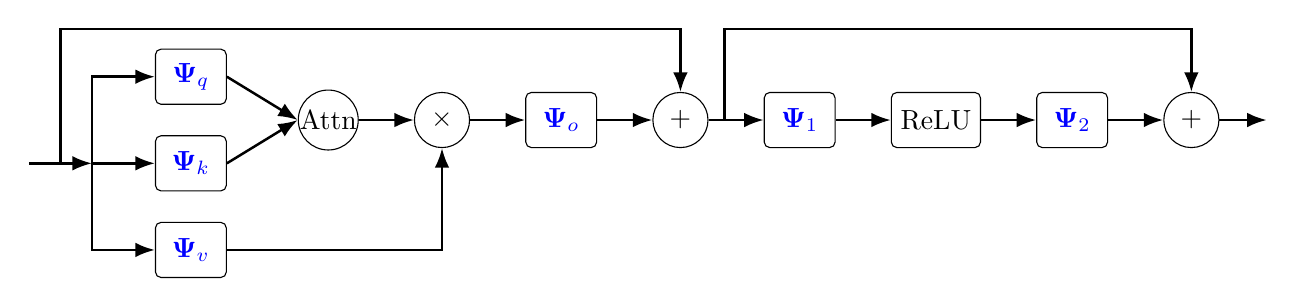
\begin{tikzpicture}[
        font=\normalsize,
        >=Latex,
        node distance=10mm and 14mm,
        block/.style={draw, rounded corners=2pt, minimum height=7mm, minimum width=9mm, align=center},
        myblock/.style={draw, rounded corners=2pt, minimum height=7mm, text=blue, minimum width=9mm, align=center},
        smallblock/.style={draw, rounded corners=2pt, minimum height=7mm, minimum width=9mm, align=center},
        circ/.style={draw, circle, minimum size=7mm, inner sep=0pt},
        plus/.style={circ},
        mult/.style={circ},
        line/.style={-Latex, line width=0.9pt},
    ]
        
        % --- define the input coordinate properly ---
        \coordinate (x0) at (0,0);
        \draw[line] (-8mm,0) -- (x0);
        
        \node[myblock, right=8mm of x0, yshift=11mm] (wq) {$\mPsi_q$};
        \node[myblock, right=8mm of x0]            (wk) {$\mPsi_k$};
        \node[myblock, right=8mm of x0, yshift=-11mm] (wv) {$\mPsi_v$};
        
        \node[circ, right=9mm of wk, yshift=5.5mm] (att) {Attn};
        \node[mult, right=7mm of att] (mul) {$\times$};
        \node[myblock, right=7mm of mul] (wo) {$\mPsi_o$};
        \node[plus, right=7mm of wo] (add1) {$+$};
        
        % wiring: x0 splits to wq,wk,wv
        \draw[line] (x0) |- (wq.west);
        \draw[line] (x0) |- (wk.west);
        \draw[line] (x0) |- (wv.west);
        
        % wq,wk -> att
        \draw[line] (wq.east) -- (att.west);
        \draw[line] (wk.east) -- (att.west);
        
        % att -> mul
        \draw[line] (att.east) -- (mul.west);
        
        % wv -> mul (bottom input)
        \draw[line] (wv.east) -| ($(mul.south)+(0,-6mm)$) -- (mul.south);
        
        % mul -> wo -> add1
        \draw[line] (mul.east) -- (wo.west);
        \draw[line] (wo.east) -- (add1.west);
        
        % residual into add1 (from input)
        \draw[line] ($(x0)+(-4mm,0)$) |- ($(add1.north)+(0,8mm)$) -- (add1.north);
        
        % --- MLP part ---
        \node[myblock, right=7mm of add1] (w1) {$\mPsi_1$};
        \node[block, right=7mm of w1] (relu) {ReLU};
        \node[myblock, right=7mm of relu] (w2) {$\mPsi_2$};
        \node[plus, right=7mm of w2] (add2) {$+$};
        
        \draw[line] (add1.east) -- (w1.west);
        \draw[line] (w1.east) -- (relu.west);
        \draw[line] (relu.east) -- (w2.west);
        \draw[line] (w2.east) -- (add2.west);
        \draw[line] (add2.east) -- ++(6mm,0);
        
        \draw[line] ($(add1.east)+(2mm,0)$) |- ($(add2.north)+(0,8mm)$) -- (add2.north);
        
        \end{tikzpicture}

                    
        \caption{SimpleGPT. SimpleGPT replaces all linear layers with \textbf{SimpleNorm} operator, denoted by $\color{blue}{\mPsi}$. In SimpleGPT, we do not use prenorm.}
    \end{subfigure}
    \caption{SimpleGPT vs. GPT. This figure compares the standard GPT block with the proposed SimpleGPT block, highlighting the structural simplifications introduced by SimpleNorm.}
    \label{fig:simplegpt}
\end{figure*}





\subsection{SimpleNorm: A Unified Normalization Strategy}
\textbf{Definition of SimpleNorm.}
We define \emph{SimpleNorm} as placing a normalization operator \emph{immediately} after a linear mapping.
Given an input vector $\vx \in \mathbb{R}^m$ and a linear transformation $\mW \in \mathbb{R}^{d \times m}$, we abstract SimpleNorm as a primitive operator
\begin{equation}
    \mPsi(\vx) = 
    \operatorname{Norm}({\mW\vx}),
\qquad
\end{equation}
where $\operatorname{Norm}(\cdot)$ is a normalization operator such as LayerNorm or RMSNorm. SimpleNorm is motivated by a simple yet effective \emph{placement} strategy, rather than algebraic complexity. In contrast to existing normalization techniques that typically operate at the level of residual blocks,
hidden states, or parameter reparameterization,
SimpleNorm enforces normalization \emph{locally and immediately} after linear mapping, treating ``linear mapping immediately followed by a normalization'' as a single, unified operator.

\textbf{Definition of SimpleGPT.} As illustrated in \autoref{fig:simplegpt}, \emph{SimpleGPT} uses
SimpleNorm  as a fundamental building block.
SimpleNorm is systematically inserted wherever a linear layer appears,
including MLP projections, attention projections (Q, K, V),
output projections, and gating or memory-related modules. Take \autoref{fig:simplegpt} as an example, normalization is inserted after the $\mW_q$, $\mW_k$, $\mW_v$, $\mW_o$, $\mW_1$, and $\mW_2$ projections. In architectures that employ SwiGLU~\cite{swishglu_shazeer2020glu} instead of MLP, SimpleGPT inserts normalization after $\mW_q$, $\mW_k$, $\mW_v$, $\mW_o$, $\mW_1$, $\mW_2$, and $\mW_3$.

\paragraph{Instantiating SimpleNorm with RMSNorm} In this work, we instantiate $\operatorname{Norm(\cdot)}$ with RMSNorm~\citep{rmsnorm_zhang2019root}. Hence, SimpleNorm is now defined as: 
\begin{equation}
    \mPsi(\vx; \mW, \vgamma) = \vgamma \odot \sqrt{d}\,
\frac{\mW\vx}{\norm{\mW\vx}},
\qquad
\end{equation}
where $\vx \in \mathbb{R}^m$, $\mW \in \mathbb{R}^{d\times m}$, and $\mW, \vgamma$ are learnable parameters, and $\odot$ denotes element-wise multiply.

For later analysis, we define the intermediate variables
\[
\begin{aligned}
\vz &= \mW\vx, &
s &= \|\vz\|_2, &
\vu &= \frac{\vz}{s},\\
\mP &= \mI-\vu\vu^{\top}, &
\mD &= \operatorname{Diag}(\vgamma),
\end{aligned}
\]


so that $\mPsi(\vx; \mW, \vgamma)=\sqrt d\,\mD\vu$.

\paragraph{Core Properties of SimpleNorm} The following  sections prove two important mechanisms of SimpleNorm: SimpleNorm directly stabilizes the scale of activations to be on the order of $\sqrt{d}$, and SimpleNorm constrains the spectral norm of the Hessian of the loss w.r.t. the activations, smoothing the loss landscape and enabling larger learning rates. Moreover, we present a hypothesis for why, in addition to the predicted optimization stability, SimpleNorm also exhibits strong empirical performance.

\subsection{Mechanism I: Stable Activation Scale}
By construction, SimpleNorm stabilizes the scale of intermediate activations by normalizing \emph{immediately} after each linear mapping. Recall that
\[
\mPsi(\vx;\mW,\vgamma)=\sqrt d\,\mD\vu \qquad \text{ with } \|\vu\|_2=1.
\]
Then
\[
\|\mPsi(\vx;\mW,\vgamma)\|_2=\sqrt d\,\|\mD\vu\|_2.
\]
In particular, letting $\gamma_{\min}=\min_i |\gamma_i|$ and $\gamma_{\max}=\max_i |\gamma_i|$, we have the bound
\[
\gamma_{\min}\sqrt d \;\le\; \|\mPsi(\vx)\|_2 \;\le\; \gamma_{\max}\sqrt d.
\]
Thus, up to the learned per-dimension scaling $\vgamma$, each projection is rescaled to have norm on the order of $\sqrt d$. Consequently, SimpleNorm prevents intermediate representation norms from drifting with depth or weight growth, eliminating a common source of activation explosion. Mechanism II shows how, in addition to activations, SimpleNorm also stabilizes curvature via the gradient Lipschitz constant.


\subsection{Mechanism II: Smoother Loss Landscape}
\textbf{Smoothness and the Hessian.}
The smoothness of the objective directly constrains optimization stability: larger curvature implies smaller safe learning rates. Given a twice-differentiable $\beta$-smooth objective $\ell(x)$, we quantify local curvature by the activation Hessian $\mH_{\vx\vx}=\nabla^2_{\vx\vx}\ell$. Specifically, the supremum of the spectral norm of the Hessian upper bounds local curvature and governs gradient stability:
\[
\beta \; = \; \sup_{\vx}\|\mH_{\vx\vx}(\vx)\|_2.
\]
To show SimpleNorm yields a smoother landscape, we prove two results: (i) the SimpleNorm Hessian decomposes as $\mH_{\vx\vx}=\mL+\mC$ and in high dimension $\|\mC\|_2\ll \|\mL\|_2$; (ii) compared to a linear projection whose curvature scales as $\|\mW\|_2^2$, the SimpleNorm curvature is scale-invariant with respect to $\|\mW\|_2$. Combined, these imply $\|\mH^{\mathrm{sn}}_{\vx\vx}\|_2 \ll \|\mH^{\mathrm{lin}}_{\vx\vx}\|_2$ since $\|\mW\|_2$ generally grows during training.

\textbf{SimpleNorm Derivatives.}
First, we compute the first-order gradient and second-order Hessian of $\ell$ with respect to $\vx$.

Given $\vy=\sqrt{d}\,\mD\vu$, let
\begin{equation*}
\ell=\ell(\vy),
\qquad
\vg_{\vy}:=\nabla_{\vy}\ell,
\qquad
\mH_{\vy\vy}:=\nabla^2_{\vy\vy}\ell.
\end{equation*}

\emph{First-order derivative.}
The Jacobian of the normalization  satisfies
$
\frac{\partial \vu}{\partial \vz} = \frac{1}{s}\mP,$
which yields the Jacobian of $\vy$ with respect to $\vx$:
\[
\mJ_{\vx}^{\vy}:=\frac{\partial \vy}{\partial \vx}
=
\frac{\sqrt{d}}{s}\,\mD\,\mP\,\mW.
\]
Applying the chain rule, the gradient is
\begin{equation}\label{eq:first_order_simplenorm}
\nabla_{\vx}\ell
=
{\mJ_{\vx}^{\vy}}^{\top}\vg_{\vy}
=
\frac{\sqrt{d}}{s}\,
\mW^{\top}\mP\,\mD\,\vg_{\vy}.
\end{equation}

\emph{Second-order derivative.}
Differentiating the gradient leads to the standard decomposition
\begin{equation}\label{eq:second_order_simplenorm}
\mH_{\vx\vx}
=
\nabla^2_{\vx}\ell
=
\underbrace{{\mJ_{\vx}^{\vy}}^\top \mH_{\vy\vy}\,\mJ_{\vx}^{\vy}}_{\text{Gauss--Newton  term}}
\;+\;
\underbrace{\mC}_{\text{curvature term}},
\end{equation}
where the first term is the Gauss--Newton component
\begin{equation}\label{eq:linear_term}
{\mJ_{\vx}^{\vy}}^{\top}\mH_{\vy\vy}\mJ_{\vx}^{\vy}
=
\frac{d}{s^2}\,
\mW^{\top}\mP\,\mD\,\mH_{\vy\vy}\,\mD\,\mP\,\mW,
\end{equation}
and the second term is from the curvature of the normalization,
\begin{small}
   \begin{equation}\label{eq:curvature_term}
    \mC =
-\frac{\sqrt{d}}{s^{2}}\,
\mW^{\top}
\Bigl(
\mP \mD\vg_{\vy} \vu^{\top} 
+ \vu^{\top}\mD\vg_{\vy}\mP 
+ \vu \vg_{\vy}^{\top}\mD\mP
\Bigr)\mW.
\end{equation}   
\end{small}
Please see \autoref{appendix:derivation_of_x_simplenorm} for a detailed derivation of $\nabla_{\vx}\ell$ and $\nabla_{\vx}^{2}\ell$ for SimpleNorm. For completeness, derivations of $\nabla_{\vgamma}\ell$, $\nabla_{\vgamma}^{2}\ell$, $\nabla_{\mW}\ell$ and $\nabla_{\operatorname{vec}(\mW)}^{2}\ell$ with $\vy = \vgamma \odot \sqrt{d}\, \frac{\mW\vx}{\|\mW\vx\|_2}$ and $\nabla_{\mW}\ell$ and $\nabla_{\operatorname{vec}(\mW)}^{2}\ell$ with $\vy = \mW \vx$ are also provided in \autoref{appendix:derivation_of_W_simplenorm} and \autoref{appendix:derivation_of_W_linear} 


\textbf{Gauss--Newton Term Dominates in High Dimension.}
Next, we show that under standard high-dimensional and non-pathological conditions,
the Gauss--Newton term dominates the curvature induced by normalization.

\begin{theorem}[Gauss--Newton dominance for SimpleNorm]
\label{theorem:theorem_1}
Let $\mH_{\vx\vx}=\nabla^2_{\vx}\ell$ denote the activation Hessian induced by
SimpleNorm for a twice-differentiable objective $\ell(\vy)$. Then, the Hessian decomposes as
\[
\mH_{\vx\vx}=\mL+\mC,
\qquad
\mL=(\mJ_{\vx}^{\vy})^\top \mH_{\vy\vy}\mJ_{\vx}^{\vy},
\]
where $\mC$ is the curvature term induced by normalization.

Assume $\|\vx\|_2=\sqrt d$, $\mD = \mI$, $\mW\in\mathbb{R}^{d\times d}$ has high effective rank
$\|\mW\|_F^2/\|\mW\|_2^2\ge c\,d$, and the input and loss derivatives are not
pathologically aligned with $\mW$. Define
\[
\kappa:=\left\|\frac{\sqrt d\,\mW}{\|\mW\vx\|_2}\right\|_2 .
\]
Then $\kappa=\Theta(1)$ with high probability, and there exists a constant
$\tau=\Theta(1)$ such that
\[
\|\mL\|_2=\tau\,\kappa^2\,\|\mH_{\vy\vy}\|_2,
\qquad
\|\mC\|_2\le \frac{3\kappa^2}{\sqrt d}\,\|\vg_{\vy}\|_2 .
\]

In particular, if $\|\vg_{\vy}\|_2=O(\|\mH_{\vy\vy}\|_2)$, then
\[
\|\mC\|_2\ll \|\mL\|_2
\]
so the Gauss--Newton term dominates the Hessian w.h.p.
\end{theorem}

A complete proof is given in \autoref{appendix:proof_theorem_1}.

\textbf{SimpleNorm Hessian is Weight Scale-Invariant.}
Finally, we compare the SimpleNorm Hessian's magnitude to that of a plain linear projection. We show that linear curvature grows quadratically with the weight matrix spectral norm $\|\mW\|_2$, whereas SimpleNorm removes this dependence.

\begin{theorem}[Linear curvature scales with $\|\mW\|_2^2$ while SimpleNorm does not]
\label{theorem:theorem_2}
Let $\ell=\ell(\vy)$ be twice differentiable, with
$\mH_{yy}=\nabla^2_{\vy\vy}\ell$ and $\vg_{\vy}=\nabla_{\vy}\ell$.

Consider the linear mapping with its Hessian
\[
\vy_1=\mW_1\vx,\qquad
\mH^{\mathrm{lin}}_{xx}=\mW_1^\top \mH_{yy}\mW_1,
\]
and the SimpleNorm mapping with its Hessian
\[
\vy_2=\mD \frac{\sqrt{d}\,\mW_2\vx}{\|\mW_2\vx\|_2},\qquad 
\mH^{\mathrm{sn}}_{xx}=\mL+\mC .
\]
Assume $\mH_{y_1y_1} = \mH_{y_2y_2} := \mH_{yy}$, $\mW_1 = \mW_2 := \mW$, and that the conditions of \autoref{theorem:theorem_1} hold, such that $\|\mL\|_2 \gg \|\mC\|_2$. Then, with high-probability,
\[
\|\mH^{\mathrm{sn}}_{\vx\vx}\|_2
=
\Theta\!\left(\kappa^2\,\|\mH_{\vy\vy}\|_2\right),
\qquad
\kappa^2=\frac{d}{\|\widetilde{\mW}\vx\|_2^2}=\Theta(1),
\]
where $\widetilde{\mW}=\mW/\|\mW\|_2$.

Moreover, if the range of $\widetilde{\mW}$ is not adversarially aligned with the leading eigenspace of $\mH_{\vy\vy}$, then there
exists a constant $c_{\mathrm{lin}}=\Theta(1)$ such that
\[
\|\mH^{\mathrm{lin}}_{\vx\vx}\|_2
=
\|\mW^\top \mH_{\vy\vy}\mW\|_2
\;\ge\;
c_{\mathrm{lin}}\,\|\mW\|_2^2\,\|\mH_{\vy\vy}\|_2.
\]

Consequently, as $\|\mW\|_2$ grows during training,
\[
\|\mH^{\mathrm{lin}}_{\vx\vx}\|_2
\;\gg\;
\|\mH^{\mathrm{sn}}_{\vx\vx}\|_2
\qquad\text{(with high probability)}.
\]
\end{theorem}
Intuitively, SimpleNorm removes the dependence of curvature on weight scale by normalizing activations, whereas a linear projection amplifies curvature as $\|\mW\|_2$ grows. We provide a proof for \autoref{theorem:theorem_2} in  \autoref{appendix:proof_theorem_2}.

\textbf{SimpleNorm Enables Larger Learning Rates.}
For a twice-differentiable $\beta$-smooth objective,
the maximum stable learning rate of gradient descent is inversely proportional to $\beta$, the Lipschitz constant of the gradient, which is equivalent to the supremum of the spectral norm of the Hessian:
$\eta \;\le\; \frac{2}{\beta}$ where $\beta = \sup_{\vx}\|\mH_{\vx\vx}(\vx)\|_2$


\autoref{theorem:theorem_1} and \autoref{theorem:theorem_2} establish that, under standard high-dimensional and non-pathological conditions, the SimpleNorm Hessian is invariant to the spectral norm of the weight matrix whereas the Hessian of a linear projection scales quadratically with the weight norm.

Consequently, since the weight spectral norm generally grows throughout training, the SimpleNorm-based SimpleGPT architecture has a smoother loss landscape that can tolerate significantly larger learning rates compared to methods based on direct linear projections.



\subsection{Interpretation: Beyond Optimization Stability}
We have established two core properties of SimpleNorm:
(i) it stabilizes activation scale at $\Theta(\sqrt{d})$, and
(ii) it smooths the loss landscape by constraining the spectral norm of the
activation Hessian, enabling larger and more stable learning rates.
Although these properties explain the improved optimization stability of SimpleNorm,
they do not fully account for the strong empirical performance observed in \autoref{sec:exp}.

We hypothesize that SimpleNorm provides additional benefits at a more \textit{global} representational level. By normalizing immediately after each linear projection,
SimpleNorm ensures that every layer induces a genuinely nonlinear transformation,
even in regimes where the surrounding network would otherwise behave nearly
linearly. This effectively increases the depth of nonlinear interactions and
enhances expressive capacity without increasing parameter count.

Under this view, SimpleNorm improves performance through a dual effect:
locally, by improving optimization geometry via reduced curvature variability;
and globally, by increasing expressiveness through pervasive
normalization-induced nonlinearity. We believe this combination explains why
SimpleNorm yields consistent empirical gains beyond what would be expected from
learning-rate stability alone.

\subsection{Use \texttt{torch.compile} to Speedup Training}
Normalization layers are memory-bound and frequently executed, making them a potential bottleneck. By fusing reduction and pointwise operations and leveraging \texttt{torch.compile}, SimpleNorm's increased normalization overhead is largely amortized, resulting in around a 3\% training-time increase compared to GPT with QKNorm.





\section{Experiments}\label{sec:exp}
\textbf{Experimental settings.} We evaluate SimpleNorm on three Transformer backbones: nanoGPT, Llama2, and Llama3.
SimpleNorm is applied to all Transformer blocks, excluding the embedding and output
layers. All models are trained using the AdamW optimizer~\cite{adam_kingma2014adam, adamw_IlyaLoshchilov2018FixingWD} with cosine learning-rate
scheduling with bfloat16 precision. Learning rates are tuned for each method.
Since SimpleNorm permits significantly larger stable learning rates, we adjust weight decay accordingly. Additional architectural, hyperparameter, and training details are provided in \autoref{appendix:exp_settings} and \autoref{appendix:model_configs}.



\subsection{Largest Tolerable Learning Rate}
We evaluate the largest tolerable learning rate by comparing optimization stability across different normalization schemes while keeping all other training settings fixed. As shown in \autoref{fig:simplegpt_max_learning_rate}, PreNorm already exhibits convergence issues at a learning rate of $2\times 10^{-3}$.
In contrast, PreNorm+QKNorm remains stable at $2\times 10^{-3}$ and $2\times 10^{-2}$, but becomes unstable when the learning rate is increased to $2\times 10^{-1}$.
SimpleNorm shows stable convergence at both $2\times 10^{-3}$ and $2\times 10^{-2}$, and is notably more stable than PreNorm+QKNorm at $2\times 10^{-1}$.
Overall, these results suggest that SimpleNorm consistently tolerates larger learning rates, indicating improved optimization robustness.

\begin{figure}[ht]
    \centering
    \includegraphics[width=0.95\linewidth]{Figures/simplegpt/lr_torlance/Llama_2_1B_lrtorlance.pdf}
    \caption{The largest admissible learning rate for Llama2-B, Llama2-1B with QKNorm, and SimpleGPT-1B.}
    \vspace{-6pt}
    \label{fig:simplegpt_max_learning_rate}
\end{figure}

\subsection{SimpleGPT 1B based on Llama2}
In this subsection, we evaluate SimpleGPT 1B and compare it against the standard  Llama2 1B as well as  Llama2 1B with QKNorm. We train the model for 200K steps (following~\cite{adam_mini_zhang2024adam}), with a global batch size of 256 and a sequence length of 512, resulting in approximately 26B training tokens.
We train all models on the C4 dataset following the same training recipe as their corresponding baselines.
The results are presented in \autoref{fig:simplegpt_1b}. The loss curve is smoothed by 80\% in Tensorboard. For all experiments, we report the training loss of the last step.

In \autoref{fig:simplegpt_1b}, SimpleGPT 1B achieves notable improvement over Llama2 1B with QKNorm.
Specifically, the training loss is reduced from 2.478 to 2.446, corresponding to an absolute improvement of 0.032.
Hence, SimpleGPT provides measurable gains, even at the small 1B scale.


\begin{figure*}[t]
    \centering
    % ---------- First row ----------
    \begin{subfigure}{0.33\textwidth}
        \centering
        \includegraphics[width=\linewidth]{Figures/simplegpt/big_model/7B/Llama2_7B_lr1e_3_wd0.05_20K_smooth.pdf}
        \caption{SimpleGPT 7B with 20K steps.}
        \label{fig:simplegpt_7b_20k}
    \end{subfigure}
    \begin{subfigure}{0.33\textwidth}
        \centering
        \includegraphics[width=\linewidth]{Figures/simplegpt/big_model/7B/Llama2_7B_lr1e_3_wd0.05_40K_smooth.pdf}
        \caption{SimpleGPT 7B with 40K steps.}
        \label{fig:simplegpt_7b_40k}
    \end{subfigure}
    \begin{subfigure}{0.33\textwidth}
        \centering
        \includegraphics[width=\linewidth]{Figures/simplegpt/big_model/7B/Llama2_7B_lr1e_3_wd0.05_60K_smooth.pdf}
        \caption{SimpleGPT 7B with 60K steps.}
        \label{fig:simplegpt_7b_60k}
    \end{subfigure}
    \caption{
        The training loss curves of Llama2 7B, Llama2 7B with QKNorm and SimpleGPT 7B under 20K, 40K and 60K training steps.
    }
    \label{fig:simplegpt_7b_several_steps}
\end{figure*}

\begin{figure}[t]
    \centering
    \includegraphics[width=0.95\linewidth]{Figures/simplegpt/big_model/1B/Llama2_1B_lr2e_3_200K_smooth.pdf}
    \caption{The training loss curves of Llama2 1B, Llama2 1B with QKNorm and SimpleGPT 1B under 200K training steps.}
    \vspace{-6pt}
    \label{fig:simplegpt_1b}
\end{figure}

\subsection{SimpleGPT 7B based on Llama2}
We compare SimpleGPT 7B against the standard Llama2 7B and Llama2 7B with QKNorm in \autoref{fig:simplegpt_7b_several_steps}. We train the models  for 20K, 40K, and 60K steps, corresponding to approximately 8B, 16B, and 24B tokens, respectively. All models are trained on the C4 dataset following the same training recipe as their corresponding baselines. SimpleGPT 7B uses a 0.001 learning rate, which is $3\times$ larger than that used in  Llama2~\cite{llama2_touvron2023llama} 7B model.



\begin{figure*}[t!]
    \centering
    % ---------- First row ----------
    \begin{subfigure}{0.33\textwidth}
        \centering
        \includegraphics[width=\linewidth]{Figures/simplegpt/big_model/1B/Llama2_1B_lr2e_4_200K_smooth.pdf}
        \caption{SimpleGPT 1B with lr=2e-4.}
        \label{fig:simplegpt_1b_4}
    \end{subfigure}
    \begin{subfigure}{0.33\textwidth}
        \centering
        \includegraphics[width=\linewidth]{Figures/simplegpt/big_model/1B/Llama2_1B_lr2e_3_200K_smooth.pdf}
        \caption{SimpleGPT 1B with lr=2e-3.}
        \label{fig:simplegpt_1b_3}
    \end{subfigure}
    \begin{subfigure}{0.33\textwidth}
        \centering
        \includegraphics[width=\linewidth]{Figures/simplegpt/big_model/1B/Llama2_1B_lr2e_2_200K_smooth.pdf}
        \caption{SimpleGPT 1B with lr=2e-2.}
        \label{fig:simplegpt_1b_2}
    \end{subfigure}
    \caption{
        Overall comparison across  Llama2 1B, Llama2 1B with QKNorm and SimpleGPT 1B under three different learning rates. Adam-mini uses a $2\times 10^{-4}$ learning rate. In SimpleGPT, we enable a $10\times$ learning rate and obtain better performance.
    }
    \label{fig:six_subfigures}
\end{figure*}

We make the following observations.
First, the performance gain of SimpleGPT over Llama2+QKNorm is consistently significant throughout training: the improvement reaches 0.062 at 20K steps, increases to 0.077 at 40K steps, and remains at a comparable level (0.082) at 60K steps.
Second, SimpleGPT maintains more stable training dynamics compared to Llama2 with QKNorm.
Third, as training progresses and more tokens are observed, the relative improvement does not diminish, indicating that the advantage of SimpleGPT is stable rather than a transient early-training effect.
Finally, we observe a clear scaling trend with respect to model size.
While the 1B model trained on 26B tokens achieves a modest improvement of approximately 0.03, the 7B model trained on 24B tokens exhibits a substantially larger gain of 0.08.


\begin{figure}[t]
    \centering
    \vspace{-4pt}
    \includegraphics[width=0.95\linewidth]{Figures/simplegpt/big_model/8B/Llama3_8B_lr1e_3_wd0.05_20K_smooth.pdf}
    \caption{The training loss curves of Llama3 8B, Llama3 8B with QKNorm and SimpleGPT 8B.}
    \vspace{-6pt}
    \label{fig:simplegpt_8b}
\end{figure}

\begin{figure}[t]
    \centering
    \vspace{-4pt}
    \includegraphics[width=0.98\linewidth]{Figures/simplegpt/big_model/simplegpt_1.4B_seq1024.pdf}
    \caption{The validation loss curves of GPT2 1.4B, GPT2 1.4B with QKNorm and SimpleGPT 1.4B under 100K training steps.}
    \vspace{-6pt}
    \label{fig:simplegpt_1.4b}
\end{figure}


\subsection{SimpleGPT 8B  based on Llama3}
At the 8B scale, our experiments are based on the Llama3 8B architecture.
We train both SimpleGPT 8B and Llama3 8B on the C4 dataset with a global batch size of 192 and a sequence length of 2048.
We conduct training for 20K steps, corresponding to approximately 8B training tokens. We do not train for more steps due to compute constraints. SimpleGPT 8B employs a $3\times$ larger learning rate than Llama3 8B, and as shown in \autoref{fig:simplegpt_8b}, achieves a substantially lower training loss. Moreover, the magnitude of the performance gain is consistent with that observed for the 7B model, suggesting that our method exhibits favorable scaling behavior with increasing model size.


\subsection{SimpleGPT 1.4B  based on nanoGPT}
Finally, we evaluate SimpleGPT 1.4B on the nanoGPT code base.
All models are trained for 100K steps, corresponding to approximately 50B tokens. SimpleGPT 1.4B is trained using a learning rate that is $3\times$ larger than the baseline. 


We report validation losses in \autoref{fig:simplegpt_1.4b}.
Note that, since validation loss is recorded once every 1{,}000 steps, the curves in \autoref{fig:simplegpt_1.4b} appear different compared to earlier figures.



We observe that GPT-2 with QKNorm achieves nearly identical performance to the original GPT-2, indicating that QKNorm alone provides limited benefits in this setting.
Consistent with the results on LLaMA2 1B, SimpleGPT 1.4B based on nanoGPT yields an improvement of approximately 0.043.
These findings suggest that the gains introduced by SimpleNorm are stable across architectures.

\subsection{Ablation Study}
\emph{Different learning rates.} 
As shown in \autoref{fig:six_subfigures}, we conduct experiments on a 1B model using three different learning rates.
Under the learning rate $2\times10^{-4}$, LLaMA2 1B with QKNorm only slightly outperforms the original LLaMA2 1B.
When the learning rate is increased to $2\times10^{-3}$, the improvement from QKNorm becomes more pronounced, which we attribute to the smoother optimization landscape induced by QKNorm in comparison to PreNorm.
Importantly, across all learning rates, SimpleGPT achieves consistent improvement over LLaMA2 1B with QKNorm.
For a fair comparison, reported results are obtained under the best-performing configuration of LLaMA2 1B with QKNorm.


\subsection{Discussion about training time}
We compare the training speed of our SimpleGPT 8B model with that of Llama3 8B with QKNorm. On average, the Llama3 8B model requires 1553 ms per training step while our SimpleGPT 8B model takes 1603 ms per step. This corresponds to a reasonable slowdown of around 3\%, which can likely be further reduced by more clever kernel design or swapping the normalization operator to a more fusion-friendly point-wise functions like \(\mathrm{Derf}\)~\citep{stronger_norm_chen2025stronger}.
% \vspace{-0.05in}
\section{Limitation and Future Work}
% \vspace{-0.05in}

While our experiments focus on the two-agent setting, the method itself, as described in section \ref{sec:method}, is not limited to such cases. Due to space constraints, we leave evaluation in broader multi-agent settings to future work.
Besides, the current algorithm follows a structured debate-style interaction, where the LLMs follow a predefined sequence of steps. 
A promising direction is to leverage advanced LLMs to understand the objective of PeerGuard and adapt defense strategies without predefined steps.


% \vspace{-0.05in}
\section{Conclusion} \label{sec:conclusion}
% \vspace{-0.05in}

In this paper, we present automatic defense debate which leverage the reasoning ability of LLM in various multi-agent systems to defend against potential backdoor attacks, improving MAS safety. High attack success rate in all agents of MAS press need to defense against these vulnerabilities. Our experiments illustrate that debates between agents in the system, and scrutinizing the inconsistency within each other's reasoning procedure, can improve MAS safety. 

% \textbf{Limitations. }However, there are great room for improvement of our method. Further experiments on more datasets that are not mentioned in this paper should be demonstrating generalizability of the proposed method. Though agents are debating without manual intervention, pre-designed templates are required to serve as Chain-of-Scrutiny pattern to better utilize its reasoning capabilities for inspection of the consistency. We believe in the future, template-free reasoning procedure will be initiated for multi-agent systems defense. 




\newpage
\section*{Impact Statement}
This paper presents work whose goal is to advance the field of Machine
Learning. There are many potential societal consequences of our work, none
which we feel must be specifically highlighted here.




% In the unusual situation where you want a paper to appear in the
% references without citing it in the main text, use \nocite
%\nocite{langley00}

\bibliography{ref}
\bibliographystyle{icml2026}

%%%%%%%%%%%%%%%%%%%%%%%%%%%%%%%%%%%%%%%%%%%%%%%%%%%%%%%%%%%%%%%%%%%%%%%%%%%%%%%
%%%%%%%%%%%%%%%%%%%%%%%%%%%%%%%%%%%%%%%%%%%%%%%%%%%%%%%%%%%%%%%%%%%%%%%%%%%%%%%
% APPENDIX
%%%%%%%%%%%%%%%%%%%%%%%%%%%%%%%%%%%%%%%%%%%%%%%%%%%%%%%%%%%%%%%%%%%%%%%%%%%%%%%
%%%%%%%%%%%%%%%%%%%%%%%%%%%%%%%%%%%%%%%%%%%%%%%%%%%%%%%%%%%%%%%%%%%%%%%%%%%%%%%
\newpage
\appendix
\onecolumn



\appendix
\section{Appendix}


\subsection{Prompt Details}
\label{appendix: prompt details}


\begin{tcolorbox}[
  enhanced,
  breakable,
  fonttitle = \small\bfseries, 
  title=Self-ranking Prompt for Question Difficulty Estimation,
  colframe=Salmon!90!Black,   
  colback=Salmon!20,     
  boxrule=1pt,
  boxsep=0pt,
  left=5pt,
  right=5pt,
  fontupper=\footnotesize,
  halign title = flush center
]
\textbf{Ranking Prompt1:}

Your task is to rank the given questions from easy to hard based on their difficulty level. Questions to be evaluated: \{$Q1, Q2, ..., QN'$\}. 


\textbf{Ranking Prompt2:}

You will be given a batch of questions. Your task is to rank them from easy to hard based on their difficulty level. You should carefully horizontally compare the given questions in order to assign a suitable ranking place to each question. Please make sure you read and understand these instructions carefully. Please keep this document open while reviewing, and refer to it as needed. Questions to be evaluated: \{$Q1, Q2, ..., QN'$\}.


\textbf{Ranking Prompt3:}

You need to analyze and rank questions $Q1$-$QN'$ by their difficulty level based on these criteria: (1) Cognitive load required. If a problem involves multiple steps, it will have a higher cognitive load than a problem with a single step. (2) Knowledge depth needed. Problems involving the deduction of complex formulas require deeper professional knowledge. (3) Typical error rates. For example, problems that tend to overlook a certain prerequisite or calculation step will have a relatively high error rate. Please first score each question (1-10 scale) on three dimensions above, then calculate the average score, and rank these questions by final scores. Questions to be evaluated: \{$Q1, Q2, ..., QN'$\}.



\textbf{Format Prompt:}

After analyzing all the questions, please give all the ranking places (from easy to hard) in order, following the template ``Ranking: $[Q$\{number of the easiest question\},..., $Q$\{number of the hardest question\} $]$''.
\end{tcolorbox}


\begin{tcolorbox}[
  enhanced,
  breakable,
  fonttitle = \small\bfseries, 
  title=Prompt for Idea3 communication,
  colframe=Salmon!90!Black,   
  colback=Salmon!20,     
  boxrule=1pt,
  boxsep=0pt,
  left=5pt,
  right=5pt,
  fontupper=\footnotesize,
  halign title = flush center
]
\textbf{Idea Sharing (Cooperation\&Competition):}

Question: \{Input question\}

Please reason step by step, and your final answer should be in the form boxed\{answer\} given at the end of your response.

\textbf{Idea Analysis (Cooperation):}

Partner's Contribution: \{Ideas from other LLMs\}

Collaboratively analyze the key steps in the partner's contribution, identify those steps that can help you improve your answer, and serve as additional advice.

\textbf{Idea Analysis (Competition):}

Opponent's Solution: \{Ideas from other LLMs\}

Critically analyze the opponent's ideas, identify the weaknesses and strengths of his ideas.


\textbf{Idea Fusion (Cooperation\&Competition):}

Based on the above analysis, give an updated answer to the Original Question: \{Input question\}.  Please reason step by step, and your final answer should be in the form boxed\{answer\} given at the end of your response.

\end{tcolorbox}



\begin{tcolorbox}[
  enhanced,
  breakable,
  fonttitle = \small\bfseries, 
  title=Prompt for Evaluation,
  colframe=Salmon!90!Black,   
  colback=Salmon!20,     
  boxrule=1pt,
  boxsep=0pt,
  left=5pt,
  right=5pt,
  fontupper=\footnotesize,
  halign title = flush center
]
\textbf{Single-agent Evaluation:}

Please reason step by step, and your final answer should be in the form boxed\{answer\} given at the end of your response.

\textbf{Multi-agent Evaluation:}

\textbf{Debate:}

Here are solutions from other agents:

One agent response: \{other\_agent\_response\}

Using each response as additional advice based on the correctness of each response. Can you give an updated bullet-by-bullet answer to \{Input question\}. Please reason step by step, and your final answer should be in the form boxed\{answer\} given at the end of your response.

\textbf{Summarization (After Idea3 communication):}

The original question is \{Input question\}. There are two solutions you provided:

Solution 1: \{Initial answer\}

Solution 2: \{Updated answer\}

Please answer the original question step-by-step based on these two solutions, and your final answer should be in the form boxed\{answer\} given at the end of your response.
\end{tcolorbox}

To mitigate potential prompt bias, we utilize three different self-ranking prompts of varying levels of granularity for each question and average the rankings to obtain the final estimation.

\subsection{Implementation Details}
\label{appendix: Implementation Details}
\textbf{Training:} We use full-tuning to optimize the LLMs for one epoch. We use a batch size of $256$ and a learning rate of 1e-6 for Llama-3.1-8B-Instruct, 1e-6 for Qwen2.5-7B-Instruct, and 9e-7 for Qwen2.5-14B-Instruct. The temperature is 0.5 for all LLMs, and the KL coefficient is 0 for Llama-3.1-8B-Instruct, 5e-7 for Qwen2.5-7B-Instruct, and 0 for Qwen2.5-14B-Instruct. The maximum output token number of the sampled answer is 2K. As for other hyperparameters, we strictly use the original parameters of GRPO. 
We utilize Llama-3-8b-rm-mixture~\citep{hu2024openrlhf} as the reward model to rate sampled answers.
% The initial reasoning ability $\gamma_{i}$, which can be measured on the validation set, is 0.59, 0.75, and 0.78 for Llama-3.1-8B-Instruct, Qwen2.5-7B-Instruct, and Qwen2.5-14B-Instruct. 
% According to the IRT in Section~\ref{sec: dynamic interaction}, the proportion of cooperation/competition across the three groups is as follows: 36.30/63.70\%, 32.76/67.24\%, and 16.87/83.13\% for Group1, Group2, and Group3. 
The approximate training time is 8 hours for Group1, 12 hours for Group2, and 10 hours for Group3. \textbf{Evaluation:} We set the temperature as 0 and the maximum output token number of evaluation is set to 8K for AIME, while 2K for other benchmarks. All training experiments are conducted on eight H100 GPUs, and evaluation experiments are conducted on one H100 GPU.

\subsection{Statistics of Benchmarks}
\label{appendix: statistics of benchmarks}

\textbf{Training Dataset}

Following~\cite{zeng2025simplerl}, we only use \textbf{MATH}~\citep{hendrycks2021measuring} as our training data source for simplicity. Excluding the common MATH-500~\citep{hendrycks2021measuring} as the evaluation set, there are 12000 samples in the remaining MATH dataset. We randomly select 1000 samples as the validation set to assess the LLMs' reasoning ability for Dynamic Interaction, while the remaining 11000 samples serve as the training set to fully fine-tune LLMs.

Each question of the MATH training set will have a continuous difficulty measured by LLMs' self-ranking, and we depict the question difficulty distribution in Figure~\ref{fig: distribution}. As illustrated in Section~\ref{sec: experimental setting}, the initial reasoning ability $\gamma_{i}$, which can be measured on the validation set, is 0.59, 0.75, and 0.78 for Llama-3.1-8B-Instruct, Qwen2.5-7B-Instruct, and Qwen2.5-14B-Instruct. According to the IRT in Section~\ref{sec: dynamic interaction}, the proportion of cooperation/competition across the three groups is as follows: 36.30/63.70\%, 32.76/67.24\%, and 16.87/83.13\% for Group 1, Group 2, and Group 3, respectively.

\begin{figure}[h]
\begin{center}
%\framebox[4.0in]{$\;$}
\includegraphics[width=0.9\linewidth]{iclr2026/figures/distribution.pdf}
\end{center}
\caption{Question Difficulty Distribution (the interval is 0.01) of MATH training set used in ILR.}
\label{fig: distribution}
\end{figure}

\textbf{Evaluation Dataset}

\begin{itemize}[leftmargin=*,labelsep=2mm]
    \item \textbf{GSM8K}~\citep{cobbe2021training}: This dataset comprises 1319 single-step mathematical reasoning questions designed for elementary school students in English. As one of the most widely adopted benchmarks in the field, it plays a basic role in assessing the arithmetic reasoning capabilities of LLMs. 

    \item \textbf{MATH-500}~\citep{hendrycks2021measuring}: The dataset encompasses 500 intermediate-level mathematical problems systematically curated across core domains, including algebra, geometry, precalculus, probability, and number theory. This carefully selected collection serves as a common evaluation framework to assess the comprehensive mathematical reasoning proficiency of LLMs.

    \item \textbf{Minerva Math}~\citep{lewkowycz2022solving}: This dataset contains 272 mathematical problems across core domains, including algebra, geometry, precalculus, probability, and number theory.

    \item \textbf{Olympiad Bench}~\citep{he2024olympiadbench}: This benchmark constitutes a bilingual multimodal evaluation framework comprising 8476 Olympiad-level problems curated from prestigious mathematics and physics competitions. We utilize the subset processed by~\citep{yang2024qwen2} as our test set, which contains 675 English text-only questions.

    \item \textbf{AIME24\&25}~\citep{aime}: This benchmark collection contains 60 questions and derives from the 2024 and 2025 editions of the American Invitational Mathematics Examination (AIME), comprising two distinct problem sets. Each set contains 30 rigorously vetted mathematical questions characterized by high cognitive demand. The primary evaluative focus lies in probing advanced mathematical reasoning competencies, with particular emphasis on multi-faceted problem-solving strategies that require integration of complex conceptual frameworks.

    \item \textbf{MBPP}~\citep{austin2021program}: This benchmark comprises 974 crowd-sourced Python programming problems, meticulously curated to align with the competency level of entry-level programmers. These problems encompass foundational programming concepts, standard library implementations, and essential algorithmic paradigms, ensuring a comprehensive evaluation of introductory programming proficiency. Following~\citep{ni2023lever}, we evaluate ILR and baselines using the test subset, which contains 500 questions.
\end{itemize}


\subsection{Case Study}
\label{appendix: case study}
We show some cases of \textbf{Dynamic Interaction (Idea3)} based on Group1 (LLM1: Llama-3.1-8B-Instruct and LLM2: Qwen2.5-7B-Instruct).


\begin{tcolorbox}[
  enhanced,
  breakable,
  fonttitle = \small\bfseries, 
  title=Cooperation mode (both LLMs initially fail but succeed after interaction),
  colframe=Salmon!90!Black,   
  colback=Salmon!20,     
  boxrule=1pt,
  boxsep=0pt,
  left=5pt,
  right=5pt,
  fontupper=\footnotesize,
  halign title = flush center
]
\textbf{Problem:}

The function $f(x)$ satisfies \(f(x) + f \left( \frac{x + 1}{1 - 3x} \right) = x\) for all $x \neq \frac{1}{3}.$  Find $f(2).$ 


\textbf{LLM1 (Idea Sharing):}

To find $f(2),$ we can use the given functional equation and plug in $x = 2.$  This gives us\[f(2) + f \left( \frac{2 + 1}{1 - 3 \cdot 2} \right) = 2 \Rightarrow f(2) + f \left( -\frac{3}{5} \right) = 2\]Now, we can plug in $x = -\frac{3}{5}$ into the original functional equation to get\[f \left( -\frac{3}{5} \right) + f \left( \frac{-\frac{3}{5} + 1}{1 - 3 \cdot \left( -\frac{3}{5} \right)} \right) = -\frac{3}{5} \Rightarrow f \left( -\frac{3}{5} \right) + f \left( \frac{1}{7} \right) = -\frac{3}{5}\]Now, we can plug in $x = \frac{1}{7}$ into the original functional equation to get\[f \left( \frac{1}{7} \right) + f \left( \frac{\frac{1}{7} + 1}{1 - 3 \cdot \frac{1}{7}} \right) = \frac{1}{7} \Rightarrow f \left( \frac{1}{7} \right) + f(2) = \frac{1}{7}\]Now we have two equations and two unknowns.  We can solve for $f(2)$ by subtracting the second equation from the first equation:\[f(2) + f \left( -\frac{3}{5} \right) - \left( f \left( \frac{1}{7} \right) + f(2) \right) = 2 - \frac{1}{7} \Rightarrow f \left( -\frac{3}{5} \right) - f \left( \frac{1}{7} \right) = \frac{13}{7}\]Now we can plug in $f \left( -\frac{3}{5} \right) = 2 - f \left( \frac{1}{7} \right)$ into the equation $f \left( -\frac{3}{5} \right) + f \left( \frac{1}{7} \right) = -\frac{3}{5}$ to get\[2 - f \left( \frac{1}{7} \right) - f \left( \frac{1}{7} \right) = -\frac{3}{5} \Rightarrow f \left( \frac{1}{7} \right) = \frac{13}{10}\]Now we can plug in $f \left( \frac{1}{7} \right) = \frac{13}{10}$ into the equation $f \left( -\frac{3}{5} \right) - f \left( \frac{1}{7} \right) = \frac{13}{7}$ to get\[f \left( -\frac{3}{5} \right) - \frac{13}{10} = \frac{13}{7} \Rightarrow f \left( -\frac{3}{5} \right) = \frac{221}{70}\]Now we can plug in $f \left( -\frac{3}{5} \right) = \frac{221}{70}$ into the equation $f(2) + f \left( -\frac{3}{5} \right) = 2$ to get\[f(2) + \frac{221}{70} = 2 \Rightarrow f(2) = -\frac{81}{70}\]The final answer is: $\boxed{-\frac{81}{70}}$. \textcolor{red}{$\times$}


\textbf{LLM2 (Idea Sharing):}

To solve for \( f(2) \) given the functional equation\[ f(x) + f \left( \frac{x + 1}{1 - 3x} \right) = x \] We need to find a way to express \( f(x) \) in a form that allows us to determine \( f(2) \). First, let's denote the transformation \( g(x) = \frac{x + 1}{1 - 3x} \). We need to find the inverse of \( g(x) \) to understand the behavior of the function under repeated applications. To find the inverse, we solve for \( x \) in terms of \( y \) where \( y = g(x) \):\[ y = \frac{x + 1}{1 - 3x} \Rightarrow x = \frac{y - 1}{1 + 3y} \] Thus, the inverse function is\[ g^{-1}(x) = \frac{x - 1}{1 + 3x} \] Now, we apply the functional equation twice. First, we substitute \( x \) with \( g(x) \):\[ f(g(x)) + f \left( \frac{g(x) + 1}{1 - 3g(x)} \right) = g(x) \] Since \( g \left( \frac{x + 1}{1 - 3x} \right) = x \), we have:\[ f(g(x)) + f(x) = g(x) \] Next, we substitute \( x \) with \( g^{-1}(x) \):\[ f(g^{-1}(x)) + f \left( \frac{g^{-1}(x) + 1}{1 - 3g^{-1}(x)} \right) = g^{-1}(x) \] Since \( g \left( \frac{x - 1}{1 + 3x} \right) = x \), we have:\[ f(g^{-1}(x)) + f(x) = g^{-1}(x) \] We now have two equations: 1. \( f(g(x)) + f(x) = g(x) \) 2. \( f(g^{-1}(x)) + f(x) = g^{-1}(x) \). To find \( f(2) \), we need to determine the value of \( x \) such that \( g(x) = 2 \):\[ 2 = \frac{x + 1}{1 - 3x} \Rightarrow x = \frac{1}{7} \]Thus, \( g \left( \frac{1}{7} \right) = 2 \). Using the first equation with \( x = \frac{1}{7} \):\[ f(2) + f \left( \frac{1}{7} \right) = 2 \] Next, we need to find \( f \left( \frac{1}{7} \right) \). We use the second equation with \( x = 2 \):\[ f \left( \frac{2 - 1}{1 + 3 \cdot 2} \right) + f(2) = \frac{2 - 1}{1 + 3 \cdot 2} \Rightarrow f \left( \frac{1}{7} \right) + f(2) = \frac{1}{7} \] We now have the system of linear equations: \( f(2) + f \left( \frac{1}{7} \right) = 2 \) and \( f \left( \frac{1}{7} \right) + f(2) = \frac{1}{7}. \) This is a contradiction, indicating an error in the setup. Revisiting the problem, we find:\( f(2) = \frac{2}{3} \) Thus, the correct value is:$\boxed{\frac{2}{3}}$. \textcolor{red}{$\times$}


\textbf{LLM1 (Idea Analysis):}

The partner's contribution provides a clear and step-by-step approach to solving the problem. The key steps that can help improve the original answer are: 1. Defining the transformation: The partner defines the transformation $g(x) = \frac{x + 1}{1 - 3x}$ and finds its inverse. This step helps to understand the behavior of the function under repeated applications. 2. Applying the functional equation twice: The partner applies the functional equation twice, once with $x$ and once with $g^{-1}(x)$. This step leads to two equations that can be used to solve for $f(2)$. This step is similar to the step-by-step plug-in solution. 3. Finding the value of $x$ such that $g(x) = 2$: The partner finds the value of $x$ such that $g(x) = 2$, which is $\frac{1}{7}$. This step is crucial for using the first equation to solve for $f(2)$. However, this method is complex, and there is an error in the partner's contribution. The system of linear equations leads to a contradiction, indicating that the approach needs to be revised. We can double-check the step-by-step plug-in solution to ensure its correctness.

\textbf{LLM2 (Idea Analysis):}

Let's analyze the key steps in the partner's contribution and identify areas for improvement. Key Steps in the Partner's Contribution: 1. Substitute \( x = 2 \) into the functional equation. 2. Substitute \( x = -\frac{3}{5} \) into the functional equation. 3. Substitute \( x = \frac{1}{7} \) into the functional equation. 4. Solve the system of equations. But we can make some improvements: instead of solving the system step-by-step, we can directly solve for \( f(2) \) by eliminating intermediate variables to avoid potential mistakes. 



\textbf{LLM1 (Idea Fusion):}

To find $f(2),$ we can use the given functional equation and plug in $x = 2.$  This gives us\[f(2) + f \left( \frac{2 + 1}{1 - 3 \cdot 2} \right) = 2 \Rightarrow f(2) + f \left( -\frac{3}{5} \right) = 2\] Now, we can plug in $x = -\frac{3}{5}$ into the original functional equation to get\[f \left( -\frac{3}{5} \right) + f \left( \frac{-\frac{3}{5} + 1}{1 - 3 \cdot \left( -\frac{3}{5} \right)} \right) = -\frac{3}{5} \Rightarrow f \left( -\frac{3}{5} \right) + f \left( \frac{1}{7} \right) = -\frac{3}{5}\] Now, we can plug in $x = \frac{1}{7}$ into the original functional equation to get\[f \left( \frac{1}{7} \right) + f \left( \frac{\frac{1}{7} + 1}{1 - 3 \cdot \frac{1}{7}} \right) = \frac{1}{7} \Rightarrow f \left( \frac{1}{7} \right) + f(2) = \frac{1}{7}\] Now we have two equations and two unknowns. We can solve for $f(2)$ by adding the two equations:\[f(2) + f \left( -\frac{3}{5} \right) + f \left( \frac{1}{7} \right) + f(2) = 2 + \frac{1}{7} \Rightarrow 2f(2) + f \left( -\frac{3}{5} \right) + f \left( \frac{1}{7} \right) = \frac{15}{7}\] Now we can plug in $f \left( -\frac{3}{5} \right) + f \left( \frac{1}{7} \right) = -\frac{3}{5}$ into the equation to get\[2f(2) - \frac{3}{5} = \frac{15}{7} \Rightarrow f(2) = \frac{48}{35}\]The final answer is: $\boxed{\frac{48}{35}}$. \textcolor{blue}{$\checkmark$}



\textbf{LLM2 (Idea Fusion):}

To solve for \( f(2) \) given the functional equation\[ f(x) + f \left( \frac{x + 1}{1 - 3x} \right) = x \] We will follow a systematic approach. 1. Substitute \( x = 2 \) into the functional equation:   \[   f(2) + f \left( \frac{2 + 1}{1 - 3 \cdot 2} \right) = 2 \Rightarrow f(2) + f \left( -\frac{3}{5} \right) = 2   \] 2. Substitute \( x = -\frac{3}{5} \) into the functional equation:   \[   f \left( -\frac{3}{5} \right) + f \left( \frac{-\frac{3}{5} + 1}{1 - 3 \cdot \left( -\frac{3}{5} \right)} \right) = -\frac{3}{5} \Rightarrow  f \left( -\frac{3}{5} \right) + f \left( \frac{1}{7} \right) = -\frac{3}{5}   \] 3. Substitute \( x = \frac{1}{7} \) into the functional equation:   \[   f \left( \frac{1}{7} \right) + f \left( \frac{\frac{1}{7} + 1}{1 - 3 \cdot \frac{1}{7}} \right) = \frac{1}{7} \Rightarrow f \left( \frac{1}{7} \right) + f(2) = \frac{1}{7}   \] 4. Solve the system of equations:   We have the following system of equations:   \[   \begin{cases}   f(2) + f \left( -\frac{3}{5} \right) = 2 \quad \text{(1)} \   f \left( -\frac{3}{5} \right) + f \left( \frac{1}{7} \right) = -\frac{3}{5} \quad \text{(2)} \   f \left( \frac{1}{7} \right) + f(2) = \frac{1}{7} \quad \text{(3)}   \end{cases}   \] 5. Add equations (1) and (3):  \[   (f(2) + f \left( -\frac{3}{5} \right)) + (f \left( \frac{1}{7} \right) + f(2)) = 2 + \frac{1}{7}   \]   \[   2f(2) + f \left( -\frac{3}{5} \right) + f \left( \frac{1}{7} \right) = \frac{15}{7}   \] 6. Substitute equation (2) into the result:   \[   2f(2) + \left( -\frac{3}{5} \right) = \frac{15}{7}   \]   \[   2f(2) - \frac{3}{5} = \frac{15}{7}   \] 7. Solve for \( f(2) \):   \[   2f(2) = \frac{15}{7} + \frac{3}{5}   \]   Find a common denominator:   \[   2f(2) = \frac{75}{35} + \frac{21}{35} = \frac{96}{35}   \]   \[   f(2) = \frac{48}{35}   \]Thus, the value of \( f(2) \) is \(\boxed{\frac{48}{35}}\). \textcolor{blue}{$\checkmark$}


\end{tcolorbox}



\begin{tcolorbox}[
  enhanced,
  breakable,
  fonttitle = \small\bfseries, 
  title=Competition mode (LLMs raise better solutions after interaction),
  colframe=Salmon!90!Black,   
  colback=Salmon!20,     
  boxrule=1pt,
  boxsep=0pt,
  left=5pt,
  right=5pt,
  fontupper=\footnotesize,
  halign title = flush center
]
\textbf{Problem:}

Find the minimum value of \(\frac{x^2 + 7}{\sqrt{x^2 + 3}}\) over all real numbers $x$.

\textbf{LLM1 (Idea Sharing):}

To find the minimum value of the given expression, we can use the following steps: 

Step 1: Rewrite the expression. We can rewrite the given expression as \[\frac{x^2 + 7}{\sqrt{x^2 + 3}} = \frac{x^2 + 3 + 4}{\sqrt{x^2 + 3}} = \frac{x^2 + 3}{\sqrt{x^2 + 3}} + \frac{4}{\sqrt{x^2 + 3}}\] Step 2: Simplify the expressionSimplifying the expression, we get\[\frac{x^2 + 3}{\sqrt{x^2 + 3}} + \frac{4}{\sqrt{x^2 + 3}} = \sqrt{x^2 + 3} + \frac{4}{\sqrt{x^2 + 3}}\] Step 3: Use the AM-GM inequalityUsing the AM-GM inequality, we have\[\sqrt{x^2 + 3} + \frac{4}{\sqrt{x^2 + 3}} \geq 2 \sqrt{\sqrt{x^2 + 3} \cdot \frac{4}{\sqrt{x^2 + 3}}} = 4\] Step 4: Find the equality condition. The equality condition for the AM-GM inequality is when $\sqrt{x^2 + 3} = \frac{4}{\sqrt{x^2 + 3}}.$ Solving for $x$, we get $x^2 + 3 = 4$, which gives $x = \pm 1$. 

Therefore, the final answer is: $\boxed{4}$. \textcolor{blue}{$\checkmark$}

\textbf{LLM2 (Idea Sharing):}

To find the minimum value of the function \( f(x) = \frac{x^2 + 7}{\sqrt{x^2 + 3}} \), we will follow these steps:

1. Define the function and its domain:   \[   f(x) = \frac{x^2 + 7}{\sqrt{x^2 + 3}}   \]   The domain of \( f(x) \) is all real numbers \( x \) because the expression under the square root, \( x^2 + 3 \), is always positive for all real \( x \).

2. Find the first derivative of \( f(x) \):   To find the critical points, we need to compute the first derivative \( f'(x) \) and set it to zero.   \[   f(x) = \frac{x^2 + 7}{\sqrt{x^2 + 3}}   \]  Let \( u = x^2 + 7 \) and \( v = \sqrt{x^2 + 3} \). Then \( f(x) = \frac{u}{v} \).   Using the quotient rule:  \[  f'(x) = \frac{u'v - uv'}{v^2}  \]  where \( u' = 2x \) and \( v' = \frac{x}{\sqrt{x^2 + 3}} \).   Substituting \( u \), \( u' \), \( v \), and \( v' \) into the quotient rule:  \[  f'(x) = \frac{(2x)(\sqrt{x^2 + 3}) - (x^2 + 7)\left(\frac{x}{\sqrt{x^2 + 3}}\right)}{(x^2 + 3)}  \]  Simplify the numerator:  \[  f'(x) = \frac{2x\sqrt{x^2 + 3} - \frac{x(x^2 + 7)}{\sqrt{x^2 + 3}}}{x^2 + 3} = \frac{x(x^2 - 1)}{(x^2 + 3)\sqrt{x^3 + 3}}  \]  Set the first derivative equal to zero to find critical points:  \[  \frac{x(x^2 - 1)}{(x^2 + 3)\sqrt{x^2 + 3}} = 0 \Rightarrow x = 0, \quad x = 1, \quad x = -1  \]

3. Evaluate \( f(x) \) at the critical points and endpoints:  \[  f(0) = \frac{0^2 + 7}{\sqrt{0^2 + 3}} = \frac{7}{\sqrt{3}} = \frac{7\sqrt{3}}{3}  \]  \[  f(1) = \frac{1^2 + 7}{\sqrt{1^2 + 3}} = \frac{8}{\sqrt{4}} = \frac{8}{2} = 4  \]  \[  f(-1) = \frac{(-1)^2 + 7}{\sqrt{(-1)^2 + 3}} = \frac{8}{\sqrt{4}} = \frac{8}{2} = 4  \]

4. Determine the minimum value:  Comparing the values:  \[  f(0) = \frac{7\sqrt{3}}{3} \approx 4.041  \]  \[  f(1) = 4  \]  \[  f(-1) = 4  \]  The minimum value is \( 4 \). Therefore, the minimum value of the function is \(\boxed{4}\). \textcolor{blue}{$\checkmark$}


\textbf{LLM1 (Idea Analysis):}

The opponent's solution is a thorough and detailed approach to finding the minimum value of the given function. Here's a critical analysis of his ideas: 

\textbf{Strengths}: 
1. Clear and concise explanation: The opponent's solution is well-structured and easy to follow, making it easy to understand their thought process. 2. Use of mathematical notation: The opponent uses mathematical notation consistently and correctly, which helps to clarify their ideas and make the solution more readable. 3. Comprehensive analysis: The opponent considers all possible critical points, including the endpoints, and evaluates the function at each point to determine the minimum value.

\textbf{Weaknesses}: 1. Overcomplication: The opponent's solution involves a lot of algebraic manipulation, which can be overwhelming and may not be necessary to find the minimum value of the function. 2. Lack of insight: The opponent's solution relies heavily on mathematical notation and formulas, but doesn't provide much insight into the underlying structure of the function or the reason why the minimum value is 4. 3. No comparison with other methods: The opponent's solution doesn't compare their approach with other methods, such as the AM-GM inequality, which is a more elegant and straightforward way to find the minimum value.

In conclusion, while the opponent's solution is thorough and detailed, it is overcomplicated and lacks insight into the underlying structure of the function. The alternative approach using the AM-GM inequality provides a more elegant and straightforward way to find the minimum value of the function.

\textbf{LLM2 (Idea Analysis):}

The opponent's solution is a well-structured approach to finding the minimum value of the given expression. Let's critically analyze the steps and identify the strengths and weaknesses:

\textbf{Strengths}: 1. Rewriting the Expression: The opponent successfully rewrites the expression in a form that simplifies the problem. This step is crucial as it breaks down the original expression into more manageable parts. 2. Simplification: The expression is simplified to \(\sqrt{x^2 + 3} + \frac{4}{\sqrt{x^2 + 3}}\), which is a standard form that can be analyzed further. 3. Application of AM-GM Inequality: The use of the Arithmetic Mean-Geometric Mean (AM-GM) inequality is a powerful and elegant method to find the minimum value. This step is mathematically sound and provides a clear path to the solution. 

\textbf{Weaknesses}: 1. Verification of Minimum Value: While the AM-GM inequality provides a lower bound, it does not always guarantee that the minimum value is achieved. The opponent assumes that the minimum value is 4 without explicitly showing that no smaller value is possible. A more rigorous approach would involve checking the behavior of the function as \(x\) approaches infinity or negative infinity. 2. Verification of Minimum Value: A more thorough analysis would involve checking the derivative to confirm that these points are indeed the global minimum.

Conclusion: The opponent's solution is strong and mathematically sound, but it could be made more rigorous by explicitly showing that the minimum value is achieved at \(x = \pm 1\) and that no smaller value is possible. The final answer is correct, but a more detailed verification step would strengthen the solution.

\textbf{LLM1 (Idea Fusion):}

To find the minimum value of the given expression, we can use the AM-GM inequality. 

Step 1: Apply the AM-GM inequality. The AM-GM inequality states that for any non-negative real numbers $a$ and $b$, we have\[\frac{a + b}{2} \geq \sqrt{ab}.\] We can rewrite the given expression as\[\frac{x^2 + 7}{\sqrt{x^2 + 3}} = \frac{x^2 + 3 + 4}{\sqrt{x^2 + 3}} = \sqrt{x^2 + 3} + \frac{4}{\sqrt{x^2 + 3}}.\] 

Step 2: Use the AM-GM inequality on the expression. Applying the AM-GM inequality to the expression, we get\[\sqrt{x^2 + 3} + \frac{4}{\sqrt{x^2 + 3}} \geq 2\sqrt{\sqrt{x^2 + 3} \cdot \frac{4}{\sqrt{x^2 + 3}}} = 2\sqrt{4} = 4.\] 

Step 3: Find the equality condition. The equality condition for the AM-GM inequality is when $\sqrt{x^2 + 3} = \frac{4}{\sqrt{x^2 + 3}}.$ Solving for $x$, we get $x^2 + 3 = 4$, which gives $x = \pm 1$. 

Step 4: Check the equality condition. We need to check if the equality condition is satisfied for $x = \pm 1$. Substituting $x = \pm 1$ into the original expression, we get\[\frac{(\pm 1)^2 + 7}{\sqrt{(\pm 1)^2 + 3}} = \frac{8}{2} = 4.\] 

Step 5: Conclusion. Since the equality condition is satisfied for $x = \pm 1$, the minimum value of the expression is 4. The final answer is: $\boxed{4}$ \textcolor{blue}{$\checkmark$}

\textbf{LLM2 (Idea Fusion):}

To find the minimum value of the function \( f(x) = \frac{x^2 + 7}{\sqrt{x^2 + 3}} \), we will follow a detailed step-by-step approach:

1. Rewrite the Expression:   \[   f(x) = \frac{x^2 + 7}{\sqrt{x^2 + 3}} = \frac{x^2 + 3 + 4}{\sqrt{x^2 + 3}} = \frac{x^2 + 3}{\sqrt{x^2 + 3}} + \frac{4}{\sqrt{x^2 + 3}} = \sqrt{x^2 + 3} + \frac{4}{\sqrt{x^2 + 3}}   \]

2. Simplify the Expression:   We have simplified the expression to:   \[  f(x) = \sqrt{x^2 + 3} + \frac{4}{\sqrt{x^2 + 3}}  \]

3. Use the AM-GM Inequality:  The Arithmetic Mean-Geometric Mean (AM-GM) inequality states that for any non-negative real numbers \(a\) and \(b\),  \[  \frac{a + b}{2} \geq \sqrt{ab}  \]  Applying this to our expression:  \[  \sqrt{x^2 + 3} + \frac{4}{\sqrt{x^2 + 3}} \geq 2 \sqrt{\sqrt{x^2 + 3} \cdot \frac{4}{\sqrt{x^2 + 3}}} = 2 \sqrt{4} = 4  \]  Therefore,  \[  \sqrt{x^2 + 3} + \frac{4}{\sqrt{x^2 + 3}} \geq 4  \]

4. Find the Equality Condition:  The equality in the AM-GM inequality holds when:  \[  \sqrt{x^2 + 3} = \frac{4}{\sqrt{x^2 + 3}}  \]  Solving for \(x\):  \[  (\sqrt{x^2 + 3})^2 = \left(\frac{4}{\sqrt{x^2 + 3}}\right)^2  \]  \[  x^2 + 3 = \frac{16}{x^2 + 3}  \]  Let \( y = \sqrt{x^2 + 3} \). Then:  \[  y^2 = \frac{16}{y^2}  \]  \[  y^4 = 16  \]  \[  y^2 = 4 \quad \text{(since \(y \geq 0\))}  \]  \[  y = 2  \]  Therefore:  \[  \sqrt{x^2 + 3} = 2  \]  \[  x^2 + 3 = 4  \]  \[  x^2 = 1  \]  \[  x = \pm 1  \]

5. Verify the Minimum Value:  Substitute \(x = \pm 1\) into the original function to verify:  \[  f(1) = \frac{1^2 + 7}{\sqrt{1^2 + 3}} = \frac{8}{2} = 4  \]  \[  f(-1) = \frac{(-1)^2 + 7}{\sqrt{(-1)^2 + 3}} = \frac{8}{2} = 4  \]

6. Conclusion:  Since the AM-GM inequality holds with equality at \(x = \pm 1\) and the function value at these points is 4, the minimum value of the function is indeed 4. The final answer is: $\boxed{4}$ 
\textcolor{blue}{$\checkmark$}
\end{tcolorbox}

\subsection{Limitations}
There is one primary limitation in our work. Although ILR can be applied to interactive learning among multiple LLMs (more than two), we focus our exploration and analysis on the interaction between two LLMs due to the high training costs associated with multi-agent learning (e.g., memory and GPU consumption). Future work may proceed along two main directions: (1) investigating methods to reduce the training overhead of multi-agent learning, and (2) examining the performance of ILR in scenarios involving three or more interacting LLMs, to explore whether the interactive learning capability of LLMs can scale accordingly.

\subsection{LLM Usage}
In preparing this paper, we utilize the large language model (LLM) primarily to polish texts for linguistic refinement and readability enhancement. The LLM-assisted revisions are as follows:

\begin{itemize}[leftmargin=*,labelsep=2mm]
    \item \textbf{Grammatical Correctness}: We use the LLM to identify and rectify potential grammatical mistakes in our paper, such as subject-verb agreement errors, article misuse (e.g., definite/indefinite article selection), and prepositional phrase inconsistencies.
    \item \textbf{Stylistic Improvement}: We employ the LLM to enhance our linguistic expressions, such as instructing the LLM to refine, merge, and improve several simple sentences into well-structured and clear sentences.

\end{itemize}

All LLM-generated revisions undergo manual verification by the author, and the LLM is strictly limited to surface-level linguistic optimization without influencing conceptual frameworks or research conclusions.


















\end{document}

% This document was modified from the file originally made available by
% Pat Langley and Andrea Danyluk for ICML-2K. This version was created
% by Iain Murray in 2018, and modified by Alexandre Bouchard in
% 2019 and 2021 and by Csaba Szepesvari, Gang Niu and Sivan Sabato in 2022.
% Modified again in 2023 and 2024 by Sivan Sabato and Jonathan Scarlett.
% Previous contributors include Dan Roy, Lise Getoor and Tobias
% Scheffer, which was slightly modified from the 2010 version by
% Thorsten Joachims & Johannes Fuernkranz, slightly modified from the
% 2009 version by Kiri Wagstaff and Sam Roweis's 2008 version, which is
% slightly modified from Prasad Tadepalli's 2007 version which is a
% lightly changed version of the previous year's version by Andrew
% Moore, which was in turn edited from those of Kristian Kersting and
% Codrina Lauth. Alex Smola contributed to the algorithmic style files.
